%%%%%%%%%%%%%%%%%%%%%%%%%%%%%%%%%%%%%%%%%%%%%%%%%%%%%%%%%%%%%%%%%%%%%%%%%%%%
%%                                                                        %%
%%                 Support de cours Programmation orientée objet                  %%
%%                                                                        %%
%%%%%%%%%%%%%%%%%%%%%%%%%%%%%%%%%%%%%%%%%%%%%%%%%%%%%%%%%%%%%%%%%%%%%%%%%%%%
%% Guillaume Moreau (EC Nantes)
%% création : 21/06/2004
%% dernière modification : 23/06/2004
%% historique :

%% il faut fixer l'URL base pour que les liens relatifs fonctionnent...
%% bizaremment fichu mais c'est comme ça.

\documentclass[allowframebreaks,xcolor=dvipsnames]{beamer}

\mode<presentation>
{
\usetheme{Antibes}
  % or ...

  %\setbeamercovered{transparent}
  % or whatever (possibly just delete it)
}
\useoutertheme{infolines}
\usecolortheme[named=RoyalBlue]{structure}

\uselanguage{french}
\languagepath{french}
\deftranslation[to=french]{definition}{définition}
\deftranslation[to=french]{Definition}{D\'efinition}
\deftranslation[to=french]{example}{exemple}
\deftranslation[to=french]{Example}{Exemple}
\deftranslation[to=french]{algorithm}{algorithme}
\deftranslation[to=french]{Algorithm}{Algorithme}

\setbeamertemplate{blocks}[rounded][shadow=true]
\setbeamertemplate{navigation symbols}{}
\setbeamertemplate{itemize item}[square]
\setbeamertemplate{itemize subitem}[triangle]

\usepackage[T1]{fontenc}
% or whatever

\usepackage[french]{babel}
% or whatever

\usepackage{tikz}
\usetikzlibrary{graphs}
\usetikzlibrary{graphdrawing.force}
\usetikzlibrary{arrows}
\usepackage{tikz-network}

%% pour afficher le plan à chaque début de section
%\AtBeginSection[]{
%  \begin{frame}{Plan}
%  \tiny \tableofcontents[currentsection, hideothersubsections]
%  \end{frame}
%}


%% tout ce qui est relatifs aux extraits de code
\usepackage{listings}
\usepackage{lstautogobble}
\lstloadlanguages{C++}
\lstset{% paramètres généraux des listings
	language=C++,
	basicstyle=\ttfamily\tiny, %% style général : chasse fixe, taille minimale
	keywordstyle=\color{webgreen}\bfseries, % les mots clés en vert et gras
	stringstyle=\color{blue}, % les chaines de caractères en bleu
	commentstyle=\color{webbrown},
	autogobble
}


\usepackage{myslides}

%% mes styles pour les graphes
\usepackage{graphstyle}

%\usepackage{times}
\usepackage[T1]{fontenc}
% Or whatever. Note that the encoding and the font should match. If T1
% does not look nice, try deleting the line with the fontenc.


\title[Option INFO / MADIS] % (optional, use only with long paper titles)
{Mathématiques discrètes}

\author[G. Moreau]{Guillaume Moreau\\
\texttt{guillaume.moreau@ec-nantes.fr}}
% - Use the \inst{?} command only if the authors have different
%   affiliation.

\institute[Ecole Centrale de Nantes] % (optional, but mostly needed)
{
  Ecole Centrale de Nantes
}

\date % (optional)
{Septembre 2020}

\subject{Théorie et algorithmique des graphes}


\definecolor{webgreen}{rgb}{0,.5,0}
\definecolor{webbrown}{rgb}{.6,0,0}
\definecolor{* }{rgb}{0,.5,0}
\definecolor{. }{rgb}{.6,0,0}

% option d'affiche de table des matières : http://mirror.unl.edu/ctan/macros/latex/contrib/beamer/doc/beameruserguide.pdf
% section 10.5

% Delete this, if you do not want the table of contents to pop up at
% the beginning of each subsection:
\AtBeginSection[]
{
   \begin{frame}
       \frametitle{Plan}
       \tableofcontents[sectionstyle=show/hide,subsectionstyle=show/show/hide,subsubsectionstyle=hide/hide]
   \end{frame}
}

\AtBeginSubsection[]
{
	\begin{frame}
		\frametitle{Plan}
		\tableofcontents[sectionstyle=show/hide,subsectionstyle=show/shaded/hide,subsubsectionstyle=show/show/hide]
	\end{frame}
}

\begin{document}

\begin{frame}
  \titlepage
\end{frame}

\begin{frame}[allowframebreaks]{Plan du cours}
  \tableofcontents[hideallsubsections]
  % You might wish to add the option [pausesections]
\end{frame}

% TODO ajouter un index


\section{Introduction}
% introduction à la théorie des graphes

\begin{frame}{Pourquoi étudier les graphes ?}
    \begin{itemize}
        \item Les graphes sont des objets abstraits permettant de modéliser de nombreux problèmes
        \begin{itemize}
            \item de la vie courante 
            \item algorithmiques 
        \end{itemize}
        \item Il existe de nombreux algorithmes pour résoudre ces problèmes
        \item Note : il existe de nombreux problèmes difficiles à résoudre 
    \end{itemize}
\end{frame}

\section{Définitions}
% Définitions pour commencer

\begin{frame}{Graphe}
    \begin{definition}
        Un \emph{graphe orienté} est un ensemble de \emph{sommets} connectés par des emph{arcs}. Formellement, $G=(S,A)$ avec
        \begin{itemize}
            \item $S$ un ensemble de sommets 
            \item $A$ une relation binaire sur $S$ (donc une partie de $S \times S$)
        \end{itemize}
    \end{definition}

    \begin{example}
        \begin{tikzpicture}
            \node[lettre] (1) at (0,0)  {1};
            \node[lettre] (2) at (0,-1) {2};
            \node[lettre] (3) at (1,-1) {3};
            \node[lettre] (4) at (1,0) {4};
            \node[lettre] (5) at (2,0) {5};
            \node[lettre] (6) at (2,-1) {6}; 
            \node (s) at (6,0) {6 sommets, 7 arcs};
            \draw[edge] (1) -> (4);
            \draw[edge] (1) -> (2) -> (4);
            \draw[edge] (2) -> (3);
            \draw[edge] (6) -> (5);
            \draw[edge] (4.260) -> (3.100);
            \draw[edge] (3.800) -> (4.280);
        \end{tikzpicture}
    \end{example}
\end{frame}

\begin{frame}{Graphe}
    \begin{definition}
        Un \emph{graphe non orienté} est un ensemble de \emph{sommets} connectés par des emph{arêtes}. Formellement, $G=(S,A)$ avec
        \begin{itemize}
            \item $S$ un ensemble de sommets 
            \item $A$ un ensemble de paires non-ordonnées de sommets
        \end{itemize}
    \end{definition}

    \begin{example}
        \begin{tikzpicture}
            \node[lettre] (1) at (0,0)  {1};
            \node[lettre] (2) at (0,-1) {2};
            \node[lettre] (3) at (1,-1) {3};
            \node[lettre] (4) at (1,0) {4};
            \node[lettre] (5) at (2,0) {5};
            \node[lettre] (6) at (2,-1) {6}; 
            \node (s) at (6,0) {6 sommets, 6 arêtes};
            \draw (1) -- (4);
            \draw (1) -- (2) -> (4);
            \draw (2) -- (3);
            \draw (6) -- (5);
            \draw (4) -- (3);
        \end{tikzpicture}
    \end{example}
\end{frame}

\begin{frame}{Vocabulaire}
    \begin{definition}
        Dans un graphe $G(S,A)$ orienté ou non, un sommet $y$ est dit \emph{adjacent} à $x$ si et seulement si $(x,y \in A$)
    \end{definition}
    \begin{example}
        \begin{tikzpicture}
            \node[lettre] (1) at (0,0)  {1};
            \node[lettre] (2) at (0,-1) {2};
            \node[lettre] (3) at (1,-1) {3};
            \node[lettre] (4) at (1,0) {4};
            \node[lettre] (5) at (2,0) {5};
            \node[lettre] (6) at (2,-1) {6}; 
            \draw[edge] (1) -> (4);
            \draw[edge] (1) -> (2) -> (4);
            \draw[edge] (2) -> (3);
            \draw[edge] (6) -> (5);
            \draw[edge] (4.260) -> (3.100);
            \draw[edge] (3.800) -> (4.280);
            \node (l) at (1,-2) {4 et 3 sont adjacents à 2};
        \end{tikzpicture}
        \begin{tikzpicture}
            \node[lettre] (1) at (0,0)  {1};
            \node[lettre] (2) at (0,-1) {2};
            \node[lettre] (3) at (1,-1) {3};
            \node[lettre] (4) at (1,0) {4};
            \node[lettre] (5) at (2,0) {5};
            \node[lettre] (6) at (2,-1) {6}; 
            \draw (1) -- (4);
            \draw (1) -- (2) -> (4);
            \draw (2) -- (3);
            \draw (6) -- (5);
            \draw (4) -- (3);
            \node (l) at (1,-2) {1, 4 et 3 sont adjacents à 2};
        \end{tikzpicture}

    \end{example}
\end{frame}

\begin{frame}{Vocabulaire}
    \begin{definition}
        Dans un graphe $G=(S,A)$ non orienté, le degré d'un sommet est le nombre de ses sommets adjacents
    \end{definition}
    \begin{example}
        \begin{tikzpicture}
            \node[lettre] (1) at (0,0)  {1};
            \node[lettre] (2) at (0,-1) {2};
            \node[lettre] (3) at (1,-1) {3};
            \node[lettre] (4) at (1,0) {4};
            \node[lettre] (5) at (2,0) {5};
            \node[lettre] (6) at (2,-1) {6}; 
            \draw (1) -- (4);
            \draw (1) -- (2) -> (4);
            \draw (2) -- (3);
            \draw (6) -- (5);
            \draw (4) -- (3);
            \node (l) at (6,0) {le sommet 3 est de degré 2};
            \node (ll) at (6,-1) {le sommet 3 est de degré 2};
        \end{tikzpicture}
    \end{example}
\end{frame}

\begin{frame}{Vocabulaire} 
    \begin{definition}
        Dans un graphe $G=(S,A)$ orienté, 
        \begin{itemize}
            \item le \emph{degré sortant} (ou extérieur) d'un sommet $x$, noté $\Gamma^+(x)$ est le nombre de ses sommets adjacents 
            \item le \emph{degré entrant} (ou intérieur) d'un sommet $x$, noté $\Gamma^-(x)$ est le nombre des sommets auxquels il est adjacent
        \end{itemize}
    \end{definition}
    \begin{example}
        \begin{tikzpicture}
            \node[lettre] (1) at (0,0)  {1};
            \node[lettre] (2) at (0,-1) {2};
            \node[lettre] (3) at (1,-1) {3};
            \node[lettre] (4) at (1,0) {4};
            \node[lettre] (5) at (2,0) {5};
            \node[lettre] (6) at (2,-1) {6}; 
            \draw[edge] (1) -> (4);
            \draw[edge] (1) -> (2) -> (4);
            \draw[edge] (2) -> (3);
            \draw[edge] (6) -> (5);
            \draw[edge] (4.260) -> (3.100);
            \draw[edge] (3.800) -> (4.280);
            \node (l) at (6,0) {le degré entrant de 2 est 1};
            \node (ll) at (6,-1) {le degré sortant de 2 est 2};
        \end{tikzpicture}        
    \end{example}
\end{frame}

\begin{frame}{Vocabulaire}
    \begin{definition}
        Dans un graphe $G=(S,A)$ orienté ou non, un \emph{chemin} est une séquence de sommets $s_0,...s_n$ où chaque paire de sommets consécutifs $(s_k,s_{k+1})$ appartient à $a$. 
    \end{definition}
    \begin{example}
        \begin{tikzpicture}
            \node[lettre] (1) at (0,0)  {1};
            \node[lettre] (2) at (0,-1) {2};
            \node[lettre] (3) at (1,-1) {3};
            \node[lettre] (4) at (1,0) {4};
            \node[lettre] (5) at (2,0) {5};
            \node[lettre] (6) at (2,-1) {6}; 
            \draw[oeedge] (1) -> (4);
            \draw[edge] (1) -> (2) -> (4);
            \draw[edge] (2) -> (3);
            \draw[edge] (6) -> (5);
            \draw[oeedge] (4.260) -> (3.100);
            \draw[edge] (3.800) -> (4.280);
            \node (l) at (1,-2) {$(1,4,3)$ est un chemin};
        \end{tikzpicture}
        \begin{tikzpicture}
            \node[lettre] (1) at (0,0)  {1};
            \node[lettre] (2) at (0,-1) {2};
            \node[lettre] (3) at (1,-1) {3};
            \node[lettre] (4) at (1,0) {4};
            \node[lettre] (5) at (2,0) {5};
            \node[lettre] (6) at (2,-1) {6}; 
            \draw[eedge] (1) -- (4);
            \draw (1) -- (2);
            \draw (2) -- (4);
            \draw[eedge] (2) -- (3);
            \draw (6) -- (5);
            \draw[eedge] (4) -- (3);
            \node (l) at (1,-2) {$(1,2,3,4)$ est un chemin};
        \end{tikzpicture}
    \end{example}
\end{frame}

\begin{frame}{Vocabulaire}
    \begin{definition}
        Dans un graphe $G=(S,A)$ orienté ou non, un chemin \emph{simple} est un chemin sans répétition de sommets
    \end{definition}
    \begin{definition}
        Dans un graphe $G=(S,A)$ orienté ou non, un \emph{cycle} est un chemin $(s_0,...s_n)$ où $s_0 = s_n$ et $s_0,...s_{n-1}$ sont distincts
    \end{definition}
\end{frame}

% connexité



\begin{frame}{Vocabulaire}
    \begin{definition}
        Un graphe $G=(S,A)$ \textbf{non orienté} est \emph{connexe} si et seulement si toute paire de sommets est reliée par au moins un chemin
    \end{definition}
    \begin{center}
        \includegraphics<1>[width=.49\textwidth]{fig/connexe.pdf}
        \includegraphics<2>[width=.49\textwidth]{fig/pasconnexe.pdf}
        \includegraphics<3>[width=.49\textwidth]{fig/pasconnexe2.pdf}
    \end{center}
    \visible<3>{Un graphe peut toujours être décomposé en une union disjointe de sous-graphes connexes : ses \emph{composantes connexes}.}
    \begin{definition}
        
    \end{definition}
\end{frame}

\begin{frame}{Vocabulaire}
    \begin{definition}
        Un graphe $G=(S,A)$ \textbf{orienté} est \emph{fortement connexe} si et seulement si toute paire de sommets est reliée par au moins un chemin
    \end{definition}
\end{frame}

\begin{frame}{Arbres}
    \begin{definition}
        Un \emph{arbre} est un graphe non-orienté connexe et acyclique (ne contient pas de cycle)
    \end{definition}
    \begin{example}
        \begin{center}
        \begin{tikzpicture}
            \node[lettre] (1) at (0,0)  {1};
            \node[lettre] (2) at (0,-1) {2};
            \node[lettre] (3) at (1,-1) {3};
            \node[lettre] (4) at (1,0) {4};
            \node[lettre] (5) at (2,0) {5};
            \node[lettre] (6) at (2,-1) {6};
            \draw (1) -- (2);     
            \draw (2) -- (4);
            \draw (2) -- (3);
            \draw (3) -- (6);
            \draw (6) -- (5);     
        \end{tikzpicture}\hspace{1cm}
        \begin{tikzpicture}
            \node[lettre] (1) at (0,0)  {1};
            \node[lettre] (2) at (0,-1) {2};
            \node[lettre] (3) at (1,-1) {3};
            \node[lettre] (4) at (1,0) {4};
            \node[lettre] (5) at (2,0) {5};
            \node[lettre] (6) at (2,-1) {6};
            \draw (1) -- (2);     
            \draw (2) -- (4);
            \draw (2) -- (3);
            \draw (3) -- (6);
            \draw (6) -- (5);  
            \draw (3) -- (4);    
        \end{tikzpicture}\hspace{1cm}
        \begin{tikzpicture}
            \node[lettre] (1) at (0,0)  {1};
            \node[lettre] (2) at (0,-1) {2};
            \node[lettre] (3) at (1,-1) {3};
            \node[lettre] (4) at (1,0) {4};
            \node[lettre] (5) at (2,0) {5};
            \node[lettre] (6) at (2,-1) {6};
            \draw (1) -- (2);     
            \draw (2) -- (4);
            \draw (2) -- (3);
            \draw (6) -- (5);  
        \end{tikzpicture}
    \end{center}

    \end{example}
\end{frame}

\begin{frame}{Propriétés des arbres}
    \begin{itemize}
        \item Les arbres ont des propriétés fortes qui permettent de simplifier et accélérer certains algorithmes 
        \begin{block}{Propriété}
            Dans un arbre $(S,A)$, $|S| = |A| + 1$
        \end{block}
    \end{itemize}
    \begin{example}
        \begin{center}
            \begin{tikzpicture}
                \node[lettre] (1) at (0,0)  {1};
                \node[lettre] (2) at (0,-1) {2};
                \node[lettre] (3) at (1,-1) {3};
                \node[lettre] (4) at (1,0) {4};
                \node[lettre] (5) at (2,0) {5};
                \node[lettre] (6) at (2,-1) {6};
                \draw (1) -- (2);     
                \draw (2) -- (4);
                \draw (2) -- (3);
                \draw (3) -- (6);
                \draw (6) -- (5);     
            \end{tikzpicture}
        \end{center}            
    \end{example}
\end{frame}

\begin{frame}{Forêts}
    \begin{definition}
        Une \emph{forêt} est un graphe non-orienté acyclique
    \end{definition}
    \begin{example}
        \begin{center}
        \begin{tikzpicture}
            \node[lettre] (1) at (0,0)  {1};
            \node[lettre] (2) at (0,-1) {2};
            \node[lettre] (3) at (1,-1) {3};
            \node[lettre] (4) at (1,0) {4};
            \node[lettre] (5) at (2,0) {5};
            \node[lettre] (6) at (2,-1) {6};
            \draw (1) -- (2);     
            \draw (2) -- (4);
            \draw (2) -- (3);
            \draw (6) -- (5);  
        \end{tikzpicture}
    \end{center}
    \end{example}
    \pause 
    \begin{block}{Propriété}
        Les composantes connexes des forêts sont des arbres
    \end{block}

\end{frame}


\begin{frame}{Fermeture transitive}
    \begin{definition}
        Dans un graphe, orienté ou non, un sommet $y$ est dit \emph{accessible} depuis un sommmet $x$ si et seulement si
        il existe un chemin de $x$ à $y$
    \end{definition}

    \begin{block}{Propriété}
        On peut décider si $y$ est accessible depuis $x$ grâce à un parcours en profondeur depuis $x$ en temps linéaire
    \end{block}

    \begin{definition}
        La \emph{fermeture transitive} d'un graphe $G=(S,A)$ est un graphe $G^*=(S,A^*)$ avec les mêmes sommets mais tel qu'il existe un arc $(x,y) \in A^*$ si et seulement si il existe un chemin de $x$ à $y$ dans $G$
    \end{definition}
\end{frame}

\begin{frame}{Propriétés}
\begin{block}{Propriété}
    La fermeture transitive d'un graphe non orienté connexe (respectivement orienté fortement connexe) est le graphe complet
\end{block}

\begin{block}{Propriété}
    Si on connait $G^*$, la requête d'accessibilité se fait en temps constant
\end{block}
\end{frame}

% TODO remplacer les Adj[i] par $\Gamma(i)$ dans les algos 

\begin{frame}{Calcul de la fermeture transitive dans un graphe \emph{creux}}
\begin{columns}
\begin{column}{0.5\textwidth}
    \begin{algorithmic}
        \Function{visite}{l,i}
        \State $A^*[l,i]$ \gets True 
        \For{$j \in \Gamma(i)$} 
        \If{non $A^*[l,j]$}  
            \State visite(l,j)
        \EndIf
        \EndFor
        \EndFunction
    \end{algorithmic}
\end{column}
\begin{column}{0.5\textwidth}
    \begin{algorithmic}
        \Function{fermeture transitive}{}
            \State $A^*$ = [[False,False],...[False,False]]
            \For{$i \in S$} 
                \State visite(i,i)
            \EndFor \\
        \Return $A^*$
        \EndFunction
    \end{algorithmic}
\end{column}
\end{columns}
\end{frame}

\begin{frame}{Exemple}
\begin{center}
    \input{genfig/ft0}
\end{center}
\end{frame}

\begin{frame}{Exemple : fermeture réflexo-transitive}
\begin{center}
    \input{genfig/ft1}
\end{center}
    \end{frame}

\begin{frame}{Calcul de la fermeture transitive}
\begin{itemize}
    \item La calcul se fait en ${\cal O}(nm)$ avec $n$ parcours en profondeur
    \item En pratique, $A*$ est plutôt dense... On peut faire le calcul de façon matricielle
    \item cf. algorithme de Floyd-Warshall en TD 
\end{itemize}
\end{frame}


% TODO placé là mais à déplacer après le merge 
% calcul des composantes fortement connexes 

\begin{frame}{Calcul des composantes fortements connexes : un peu d'histoire}

\begin{itemize}
    \item Années 60 : un problème classique 
    \begin{itemize}
        \item mais sans solution efficace (polynomiale)
        \item la complexité du problème n'est pas connue 
    \end{itemize}
    \item 1972 : algorithme linéaire proposé par Trojan 
    \begin{itemize}
        \item simple modification du parcours en profondeur 
        \item difficile à comprendre 
    \end{itemize}
    \item années 80 : algorithme linéaire de Kosajaru 
    \begin{itemize}
        \item plus simple à comprendre (2 parcours)
        \item la légende dit qu'il avait oublié ses notes de cours et qu'il a inventé l'algorithme en préparant son cours 
    \end{itemize}
\end{itemize}
\end{frame}

\begin{frame}{Notion de graphe inverse}
\begin{definition}
    Le graphe \emph{inverse} d'un graphe $G=(S,A)$ est le graphe $G'=(S,A')$ possédant les mêmes sommets mais possédant un arc $(i,j) \in A'$ si et seulement si $(j,i) \in A$    
\end{definition}

\begin{example}
    \begin{tikzpicture}
        \node[lettre] (1) at (0,0)  {1};
        \node[lettre] (2) at (0,-1) {2};
        \node[lettre] (3) at (1,-1) {3};
        \node[lettre] (4) at (1,0) {4};
        \node[lettre] (5) at (2,0) {5};
        \node[lettre] (6) at (2,-1) {6}; 
        \draw[edge] (1) -> (4);
        \draw[edge] (1) -> (2) -> (4);
        \draw[edge] (2) -> (3);
        \draw[edge] (6) -> (5);
        \draw[edge] (4.260) -> (3.100);
        \draw[edge] (3.800) -> (4.280);
        \node (l) at (4.5,0) { et son graphe inverse};
    \end{tikzpicture}        
    \begin{tikzpicture}
        \node[lettre] (1) at (0,0)  {1};
        \node[lettre] (2) at (0,-1) {2};
        \node[lettre] (3) at (1,-1) {3};
        \node[lettre] (4) at (1,0) {4};
        \node[lettre] (5) at (2,0) {5};
        \node[lettre] (6) at (2,-1) {6}; 
        \draw[edge] (4) -> (1);
        \draw[edge] (4) -> (2) -> (1);
        \draw[edge] (3) -> (2);
        \draw[edge] (5) -> (6);
        \draw[edge] (4.260) -> (3.100);
        \draw[edge] (3.800) -> (4.280);
    \end{tikzpicture}        
\end{example}

\begin{block}{Propriété}
    Les composantes fortement connexes d'un graphe sont identiques à celles de son graphe inverse
\end{block}

\end{frame}

\begin{frame}{Algorithme de Kosaraju : principe}

\begin{enumerate}
    \item Parcours en profondeur de $G$ pour retenir un ordre suffixe
    \begin{itemize}
        \item i.e. quand on visite $b$ depuis $a$, on note $b$, $a$
    \end{itemize}
    \item Calcul de $G'$ l'inverse de $G$
    \item Parcours en profondeur sur $G'$ mais avec modification de la boucle principale : on prend la boucle principale par l'inverse de l'ordre suffixe établi à la première étape
    \item Les composantes fortement connexes sont les arbres de la forêt du second parcours
\end{enumerate}

\end{frame}

\begin{frame}[fragile]
    \frametitle{Algorithme de Kosaraju (partie 1)}
        \begin{columns}
            \begin{column}{.5\textwidth}
                \begin{algorithmic}[1]
                    \Function{visite}{$i$ : sommet}
                    \State vu[i] \gets true
                    \For{$j \in Adj[i]$}
                        \If{$vu[j] = false$}
                            \State visite(j)
                        \EndIf
                    \EndFor
                    \State \textcolor{blue}{os.add(i)}
                    \EndFunction
                \end{algorithmic}
            \end{column}
            \begin{column}{.5\textwidth}
                \begin{algorithmic}[1]
                    \State vu \gets [$false$,...,$false$]
                    \State \textcolor{blue}{os \gets []}
                    \For{$i \in S$}
                        \If{$vu[i] = false$}
                        \State visite(i)
                        \EndIf
                    \EndFor
                    \end{algorithmic}            
            \end{column}
        \end{columns}    
    \end{frame}

    \begin{frame}[fragile]
        \frametitle{Algorithme de Kosaraju (partie 2)}
            \begin{columns}
                \begin{column}{.5\textwidth}
                    \begin{algorithmic}[1]
                        \Function{visite\_k}{ginv,$i$ : sommet,ncb}
                        \State vu[i] \gets true
                        \State cfc[i] \gets ncb
                        \For{$j \in Adj[i]$}
                            \If{$vu[j] = false$}
                                \State visite\_k(ginv,j,ncb)
                            \EndIf
                        \EndFor
                        \EndFunction
                    \end{algorithmic}
                \end{column}
                \begin{column}{.5\textwidth}
                    \begin{algorithmic}[1]
                        \While{!os.empty()}
                        \State i \gets os.pop() 
                        \If{vu[i] == False}
                            \State cfc[i] \gets ncb
                            \State visite\_k(ginv,i,ncb)
                            \State ncb \gets ncb+1
                        \EndIf
                        \EndWhile
                        \end{algorithmic}            
                \end{column}
            \end{columns}    
        \end{frame}
    
% TODO faut-il inclure l'algorithme de Tarjan à titre de comparaison ?

\begin{frame}[fragile]
\frametitle{Algorithme de Kosaraju}
\begin{pythoncode}
# Parcours en profondeur avec stockage de l'ordre suffixe 
def visite(g,i):
    global ordre_suffixe
    i["vu"] = True
    for j in g.successors(i):
        if g.vs[j]["vu"] == False:
            visite(g,g.vs[j])
    ordre_suffixe.append(i["nom"])


\end{pythoncode}
\end{frame}


\begin{frame}[fragile]
\frametitle{Algorithme de Kosaraju}
\begin{pythoncode}    
# initialisation
for s in g1.vs:
    s["vu"] = False
ordre_suffixe = []
for i in g1.vs:
    if i["vu"] == False:
        visite(g1,i)

\end{pythoncode}
\end{frame}

\begin{frame}[fragile]
\frametitle{Algorithme de Kosaraju}
\begin{pythoncode}    

#inversion du graphe 
ginv = ig.Graph(24,[],True)
n = 1
for v in ginv.vs:
    v["nom"] = str(n) 
    v["vu"] = False 
    n = n + 1
for e in g1.es: 
    ginv.add_edge(e.target,e.source)

ncb = 1

while ordre_suffixe:
    i = ordre_suffixe.pop()
    e = ginv.vs.select(nom = i)[0]
    if (e["vu"] == False):
        e["comp"] = ncb
        visite_k(ginv,e,ncb)
        ncb = ncb+1
\end{pythoncode}
\end{frame}

\begin{frame}[fragile]
    \frametitle{Algorithme de Kosaraju}
    \begin{pythoncode}   
    
    def visite_k(ginv, v, ncb):
        v["vu"] = True
        v["comp"] = ncb
        for i in v.successors():
            if i["vu"] == False:
                visite_k(ginv, i, ncb)
    \end{pythoncode}
    \end{frame}
    


% représentation des graphes 

\section{Représentation des graphes}

\begin{frame}{Représentation des graphes}
    \begin{itemize}
        \item On s'intéresse à la représentation des graphes orientés ou non
        \begin{itemize}
            \item revient au même à une redondance près
        \end{itemize}
        \item On suppose $S={1,...,n}$
        \begin{itemize}
            \item au besoin on utilise une structure de dictionnaire (map) pour faire un lien entre sommets et indexes
        \end{itemize}
    \end{itemize}
\end{frame}

\begin{frame}{Opérations de base}
    \begin{itemize}
        \item Créer un graphe à $n$ sommets, sans arcs
        \item Ajouter un arc
        \item Tester l'existence d'un arc 
        \item Parcourir les sommets adjacents à un sommet 
        \item Parcourir \textbf{tous} les sommets en explorant le graphe
        \begin{itemize}
            \item Algorithme de \emph{parcours de graphe}
        \end{itemize}
    \end{itemize}
\end{frame}

\begin{frame}{Représentation par matrice d'adjacences}
    \begin{itemize}
        \item une matrice $n \times n$ à valeurs dans $\{0,1\}$
    \end{itemize}
    \begin{equation*}
        M_{i,j} = \left\{ 
            \begin{array}{ll}
                1 & \mbox{si } (i,j) \in A \\
                0 & \mbox{sinon} \\
            \end{array}
            \right.
        \end{equation*}
\begin{itemize}
    \item Bien adapté aux graphes denses 
\end{itemize}
\end{frame}

\begin{frame}{Exemple}
    \begin{columns}
        \begin{column}{.5\textwidth}
            \begin{tikzpicture}
                \node[lettre] (1) at (1,0)  {1};
                \node[lettre] (2) at (3,-0) {2};
                \node[lettre] (3) at (3,-1) {3};
                \node[lettre] (4) at (2,-1) {4};
                \node[lettre] (5) at (0,-1) {5};
                \node[lettre] (6) at (1,-2) {6}; 
                \draw[edge] (1) -> (2);
                \draw[edge] (1) -> (4);
                \draw[edge] (1) -> (5);
                \draw[edge] (5) -> (6);
                \draw[edge] (6) -> (4);
                \draw[edge] (3) -> (4);
                \draw[edge] (2.260) -> (3.100);
                \draw[edge] (3.800) -> (2.280);
                \draw[edge] (5.10) -> (4.170);
                \draw[edge] (4.190) -> (5.350);
            \end{tikzpicture}
        \end{column}
        \begin{column}{.5\textwidth}
            \begin{equation*}
                m = \left(
                  \begin{array}{cccccc}
                    0 & 1 & 0 & 1 & 1 & 0 \\
                    0 & 0 & 1 & 0 & 0 & 0 \\
                    0 & 1 & 0 & 1 & 0 & 0 \\
                    0 & 0 & 0 & 0 & 1 & 0 \\
                    0 & 0 & 0 & 1 & 0 & 1 \\
                    0 & 0 & 0 & 1 & 0 & 0 \\
                  \end{array}
                  \right)
              \end{equation*}
        \end{column}
    \end{columns}    
\end{frame}

\begin{frame}{Exemple}
    \begin{columns}
        \begin{column}{.5\textwidth}
            \begin{tikzpicture}
                \node[lettre] (1) at (1,0)  {1};
                \node[lettre] (2) at (3,-0) {2};
                \node[lettre] (3) at (3,-1) {3};
                \node[lettre] (4) at (2,-1) {4};
                \node[lettre] (5) at (0,-1) {5};
                \node[lettre] (6) at (1,-2) {6}; 
                \draw[edge] (1) -> (2);
                \draw[edge] (1) -> (4);
                \draw[edge] (1) -> (5);
                \draw[edge] (5) -> (6);
                \draw[oeedge] (6) -> (4);
                \draw[edge] (3) -> (4);
                \draw[edge] (2.260) -> (3.100);
                \draw[edge] (3.800) -> (2.280);
                \draw[edge] (5.10) -> (4.170);
                \draw[edge] (4.190) -> (5.350);
            \end{tikzpicture}
        \end{column}
        \begin{column}{.5\textwidth}
            \begin{equation*}
                m = \left(
                  \begin{array}{cccccc}
                    0 & 1 & 0 & 1 & 1 & 0 \\
                    0 & 0 & 1 & 0 & 0 & 0 \\
                    0 & 1 & 0 & 1 & 0 & 0 \\
                    0 & 0 & 0 & 0 & 1 & 0 \\
                    0 & 0 & 0 & 1 & 0 & 1 \\
                    0 & 0 & 0 & \textcolor{blue}{\textbf{1}} & 0 & 0 \\
                  \end{array}
                  \right)
              \end{equation*}
        \end{column}
    \end{columns}    
\end{frame}

\begin{frame}{Quelques chiffres}
    \begin{itemize}
        \item $G=(S,A)$ à $n$ sommets et $m$ arcs 
        \item Dans un graphe orienté : $m \leq n^2$ 
        \begin{itemize}
            \item Si $m=n^2$, le graphe est \emph{complet}
        \end{itemize}
        \item Dans un graphe non-orienté : $m \leq \frac{n(n+1)}{2}$
        \begin{itemize}
            \item Graphe complet si égalité 
        \end{itemize}
        \item Si $m \sim  n^2$, on parle de graphe \emph{dense}
    \end{itemize}
\end{frame}

\begin{frame}{Représentation par liste d'adjacences}
    \begin{itemize}
        \item Un tableau $Adj$ de $|S|$ listes de sommets tel que pour tout sommet $i$, $Adj[i]$ contient les adjacents de $i$
        \begin{equation*}
            Adj[i] = \{  j | (i,j) \in A \}
        \end{equation*}
        \item Bien adapté aux graphes peu denses (\textit{sparse})
    \end{itemize}
\end{frame}

\begin{frame}{Exemple}
    \begin{columns}
        \begin{column}{.5\textwidth}
            \begin{tikzpicture}
                \node[lettre] (1) at (1,0)  {1};
                \node[lettre] (2) at (3,-0) {2};
                \node[lettre] (3) at (3,-1) {3};
                \node[lettre] (4) at (2,-1) {4};
                \node[lettre] (5) at (0,-1) {5};
                \node[lettre] (6) at (1,-2) {6}; 
                \draw[edge] (1) -> (2);
                \draw[edge] (1) -> (4);
                \draw[edge] (1) -> (5);
                \draw[edge] (5) -> (6);
                \draw[edge] (6) -> (4);
                \draw[edge] (3) -> (4);
                \draw[edge] (2.260) -> (3.100);
                \draw[edge] (3.800) -> (2.280);
                \draw[edge] (5.10) -> (4.170);
                \draw[edge] (4.190) -> (5.350);
            \end{tikzpicture}
        \end{column}
        \begin{column}{.5\textwidth}
            \begin{equation*}
                  \begin{array}{ccl}
                    Adj[1] & = & \{2, 4, 5 \} \\
                    Adj[2] & = & \{3 \} \\
                    Adj[3] & = & \{ 2, 4 \} \\
                    Adj[4] & = & \{ 5 \} \\
                    Adj[5] & = & \{ 4, 6 \} \\
                    Adj[6] & = & \{ 4 \} \\
                  \end{array}
              \end{equation*}
            Note : les listes sont ordonnées ici, cela n'a rien d'obligatoire
        \end{column}
    \end{columns}    
\end{frame}

\begin{frame}{Autres représentations}
    \begin{itemize}
        \item une seule liste de tous les arcs/arêtes 
        \begin{equation*}
            TA = \left[
              \begin{array}{cccccccccc}
              1 & 1 & 1 & 2 & 3 & 3 & 4 & 5 & 5 & 6 \\
              2 & 4 & 5 & 3 & 2 & 4 & 5 & 4 & 6 & 4 \\
              \end{array}
              \right]
          \end{equation*}          
        \item toute forme de compression possible 
        \begin{itemize}
            \item \textit{façon RLE}
            \begin{equation*}
                T_1 = \left[
                  \begin{array}{cccccccccc}
                  2 & 4 & 5 & 3 & 2 & 4 & 5 & 4 & 6 & 4 \\
                  \end{array}
                  \right]
              \end{equation*}
              
              \begin{equation*}
                T_2 = \left[
                  \begin{array}{cccccc}
                   1 & 4 & 5 & 7 & 8 & 10 \\
                  \end{array}
                  \right]
              \end{equation*}
              
        \end{itemize}
    \end{itemize}
    \pause 
    \alert{Dans tous les cas, les coûts de manipulation sont différents ! Il va falloir faire un compromis entre coût mémoire / coût en temps de calcul / coût en développement des algorithmes}
\end{frame}

% aborder l'efficacité des représentations 

\begin{frame}{Efficacité des représentations}
    \begin{center}
        \begin{tabular}{|l|c|c|c|}
            \hline
            Représentation & Espace & $(i,j)\in A$ ? & $\Gamma^+(a)$ \\
            \hline
            liste d'arcs & ${\cal O}(m)$ & ${\cal O}(m)$ & ${\cal O}(m)$ \\
            \hline
            matrice d'adjacences & ${\cal O}(n^2)$ & ${\cal O}(1)$ & ${\cal O}(n)$  \\
            \hline  
            tableau d'adjacences & ${\cal O}(n+m)$ & ${\cal O}(\Gamma(i))$ &  ${\cal O}(\Gamma(i))$ \\ 
            \hline
        \end{tabular}
    \end{center}

    \begin{itemize}
        \item Questions
        \begin{itemize}
            \item Que se passe-t-il si on cherche $\Gamma^-(i)$ ?
            \item Que se passe-t-il si la liste d'arcs est triée ?
        \end{itemize}
    \end{itemize}
\end{frame}

\begin{frame}{Efficacité des représentations}
    \begin{center}
        \begin{tabular}{|l|c|c|c|}
            \hline
            Représentation & Espace & $(i,j)\in A$ ? & $\Gamma^+(a)$ \\
            \hline
            liste d'arcs & ${\cal O}(m)$ & ${\cal O}(m)$ & ${\cal O}(m)$ \\
            \hline 
            \textcolor{blue}{liste triée} & ${\cal O}(m)$ & ${\cal O}(\log n + \log \Gamma^+(i))$ & ${\cal O}(\log n + \Gamma^+(i))$ \\
            \hline
            $M_{i,j}$ & ${\cal O}(n^2)$ & ${\cal O}(1)$ & ${\cal O}(n)$  \\
            \hline  
            $Adj[i]$ & ${\cal O}(n+m)$ & ${\cal O}(\Gamma(i))$ &  ${\cal O}(\Gamma(i))$ \\ 
            \hline
        \end{tabular}
    \end{center}

    \begin{itemize}
        \item En pratique, les graphes sont rarement denses 
    \end{itemize}
\end{frame}



% TODO il manque un élément de plan pour les parcours de graphe

% parcours de graphes 

\begin{frame}{Parcours de graphe}
\begin{itemize}
    \item Comment parcourir un graphe de façon exhaustive ?
    \item Explorer tous les sommets 
    \begin{itemize}
        \item En partant d'un sommet d'origine (ou plusieurs si le graphe n'est pas connexe / fortement connexe)
        \item En suivant uniquement les arcs qui sortent d'un sommet déjà exploré
        \item En construisant un historique de son parcours : notion d'arbre de \emph{parcours}
    \end{itemize}
    \item Routine de base en algorithmique des graphes 
\end{itemize}
\end{frame}

\begin{frame}{Comment ?}
    \begin{center}
        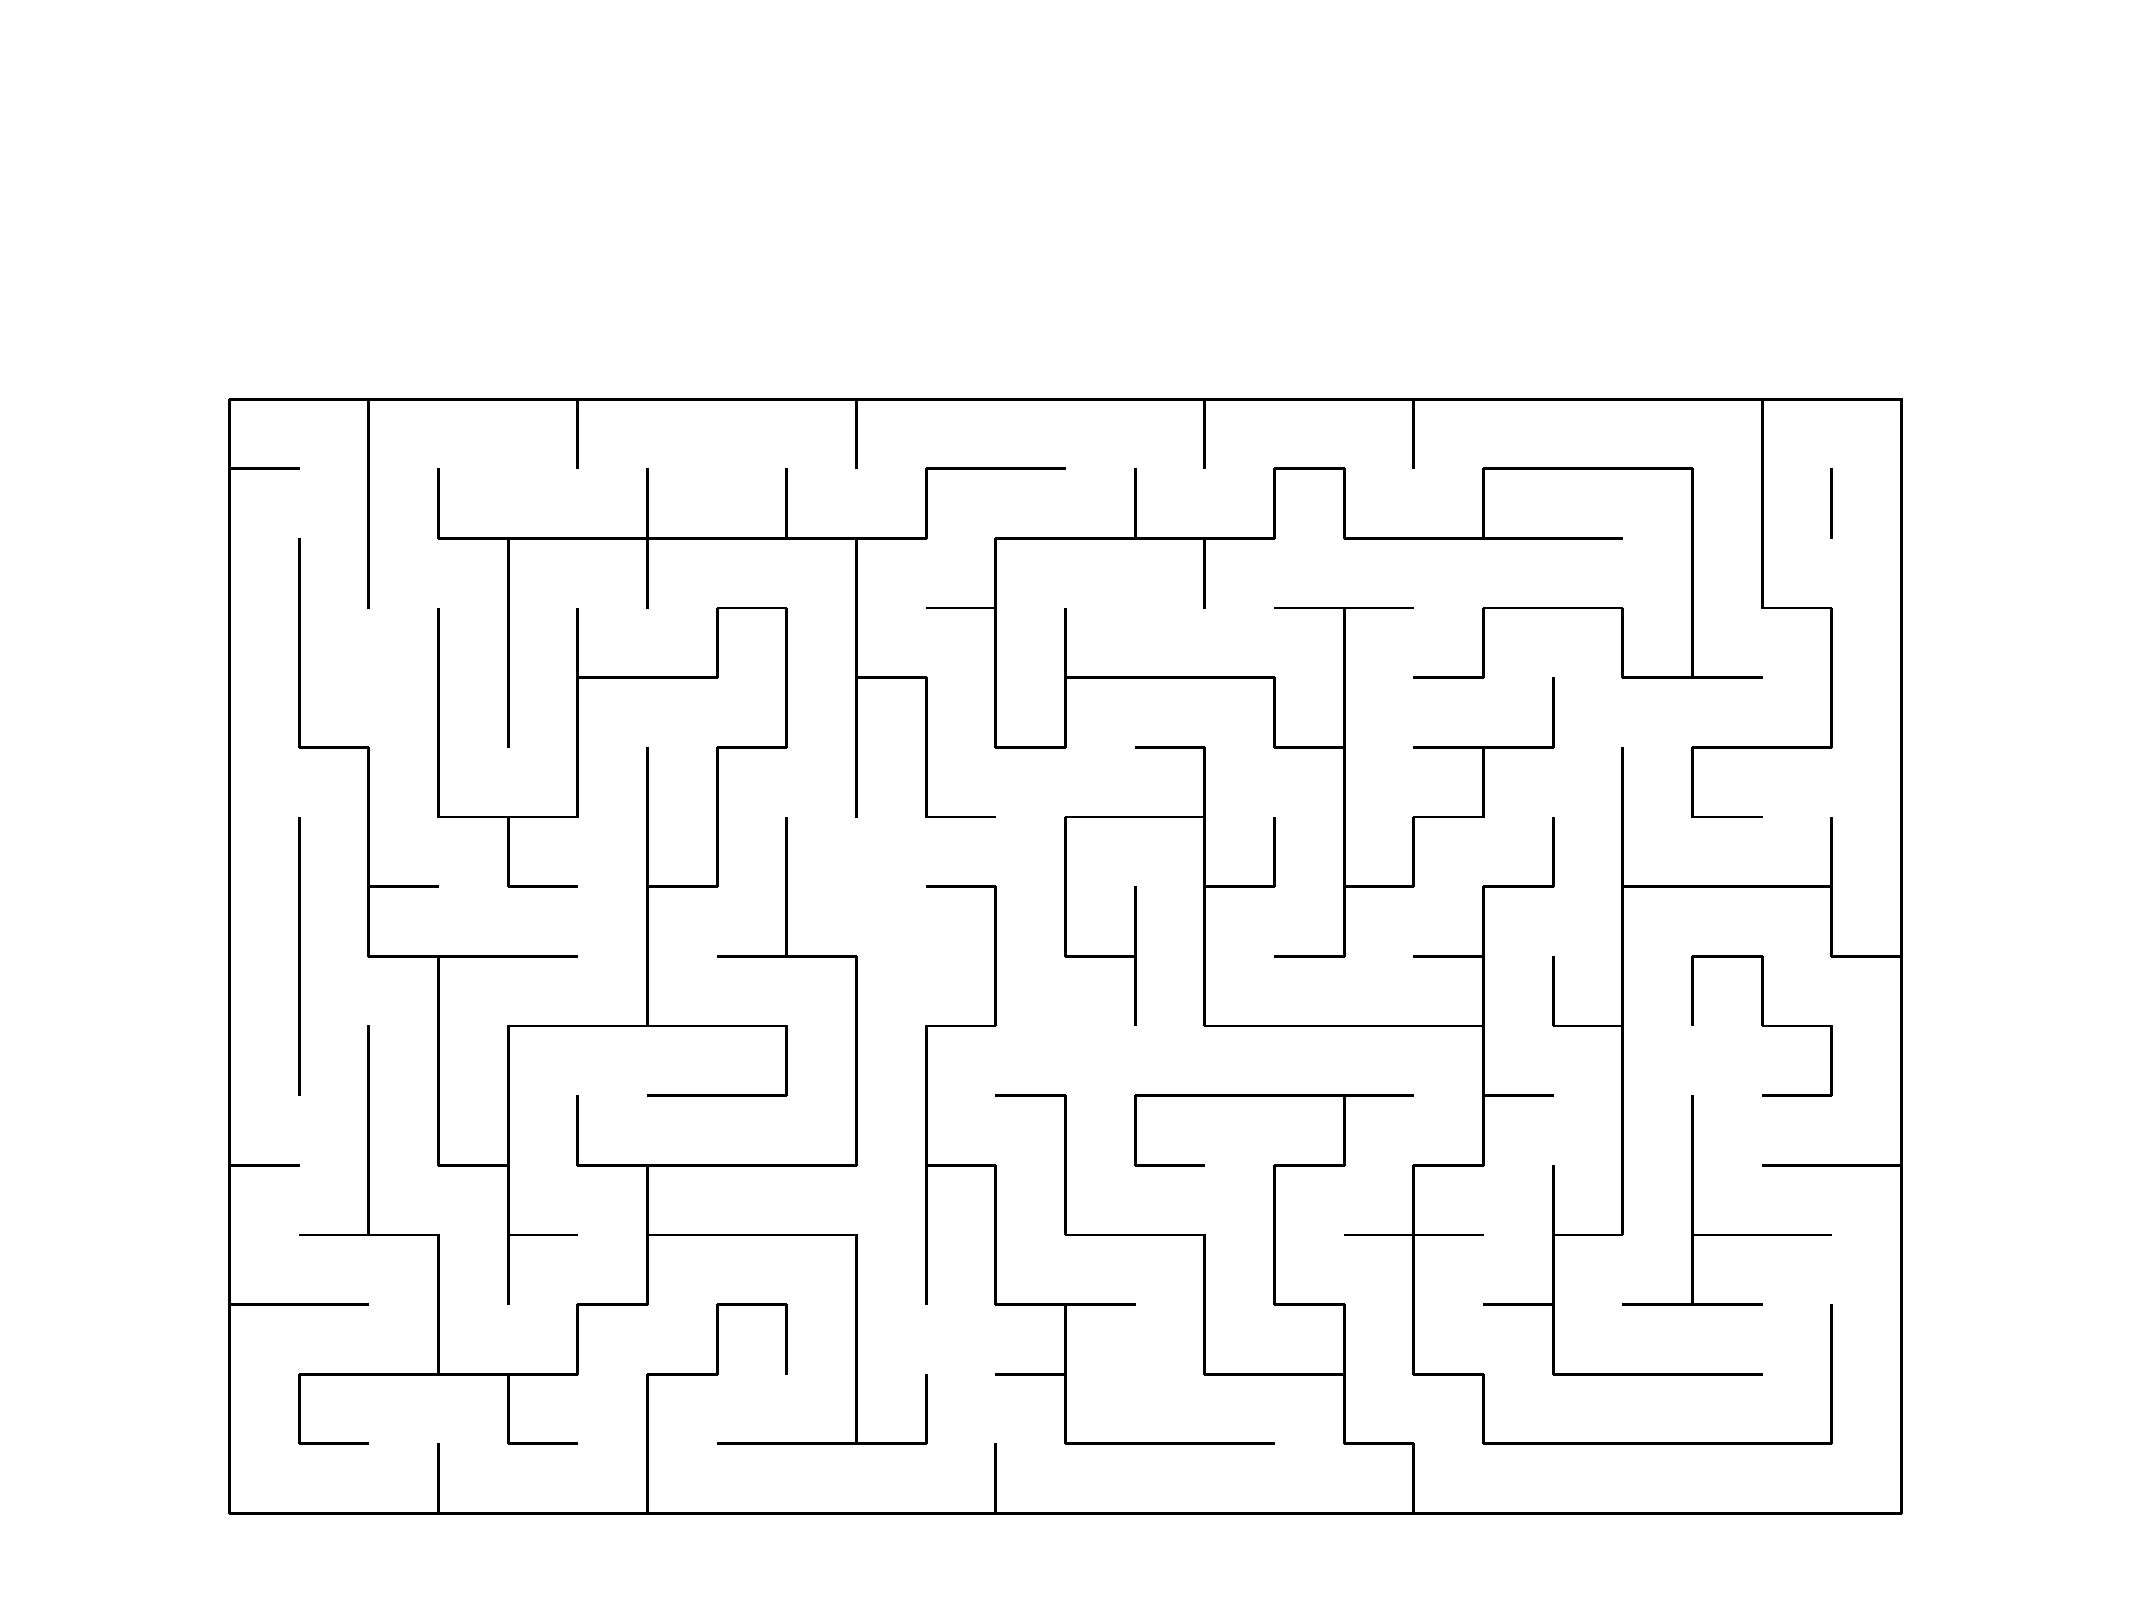
\includegraphics[width=.75\textwidth]{fig/labyrinthe.pdf}
    \end{center}
\end{frame}

\begin{frame}{Comment ?}
    \begin{center}
        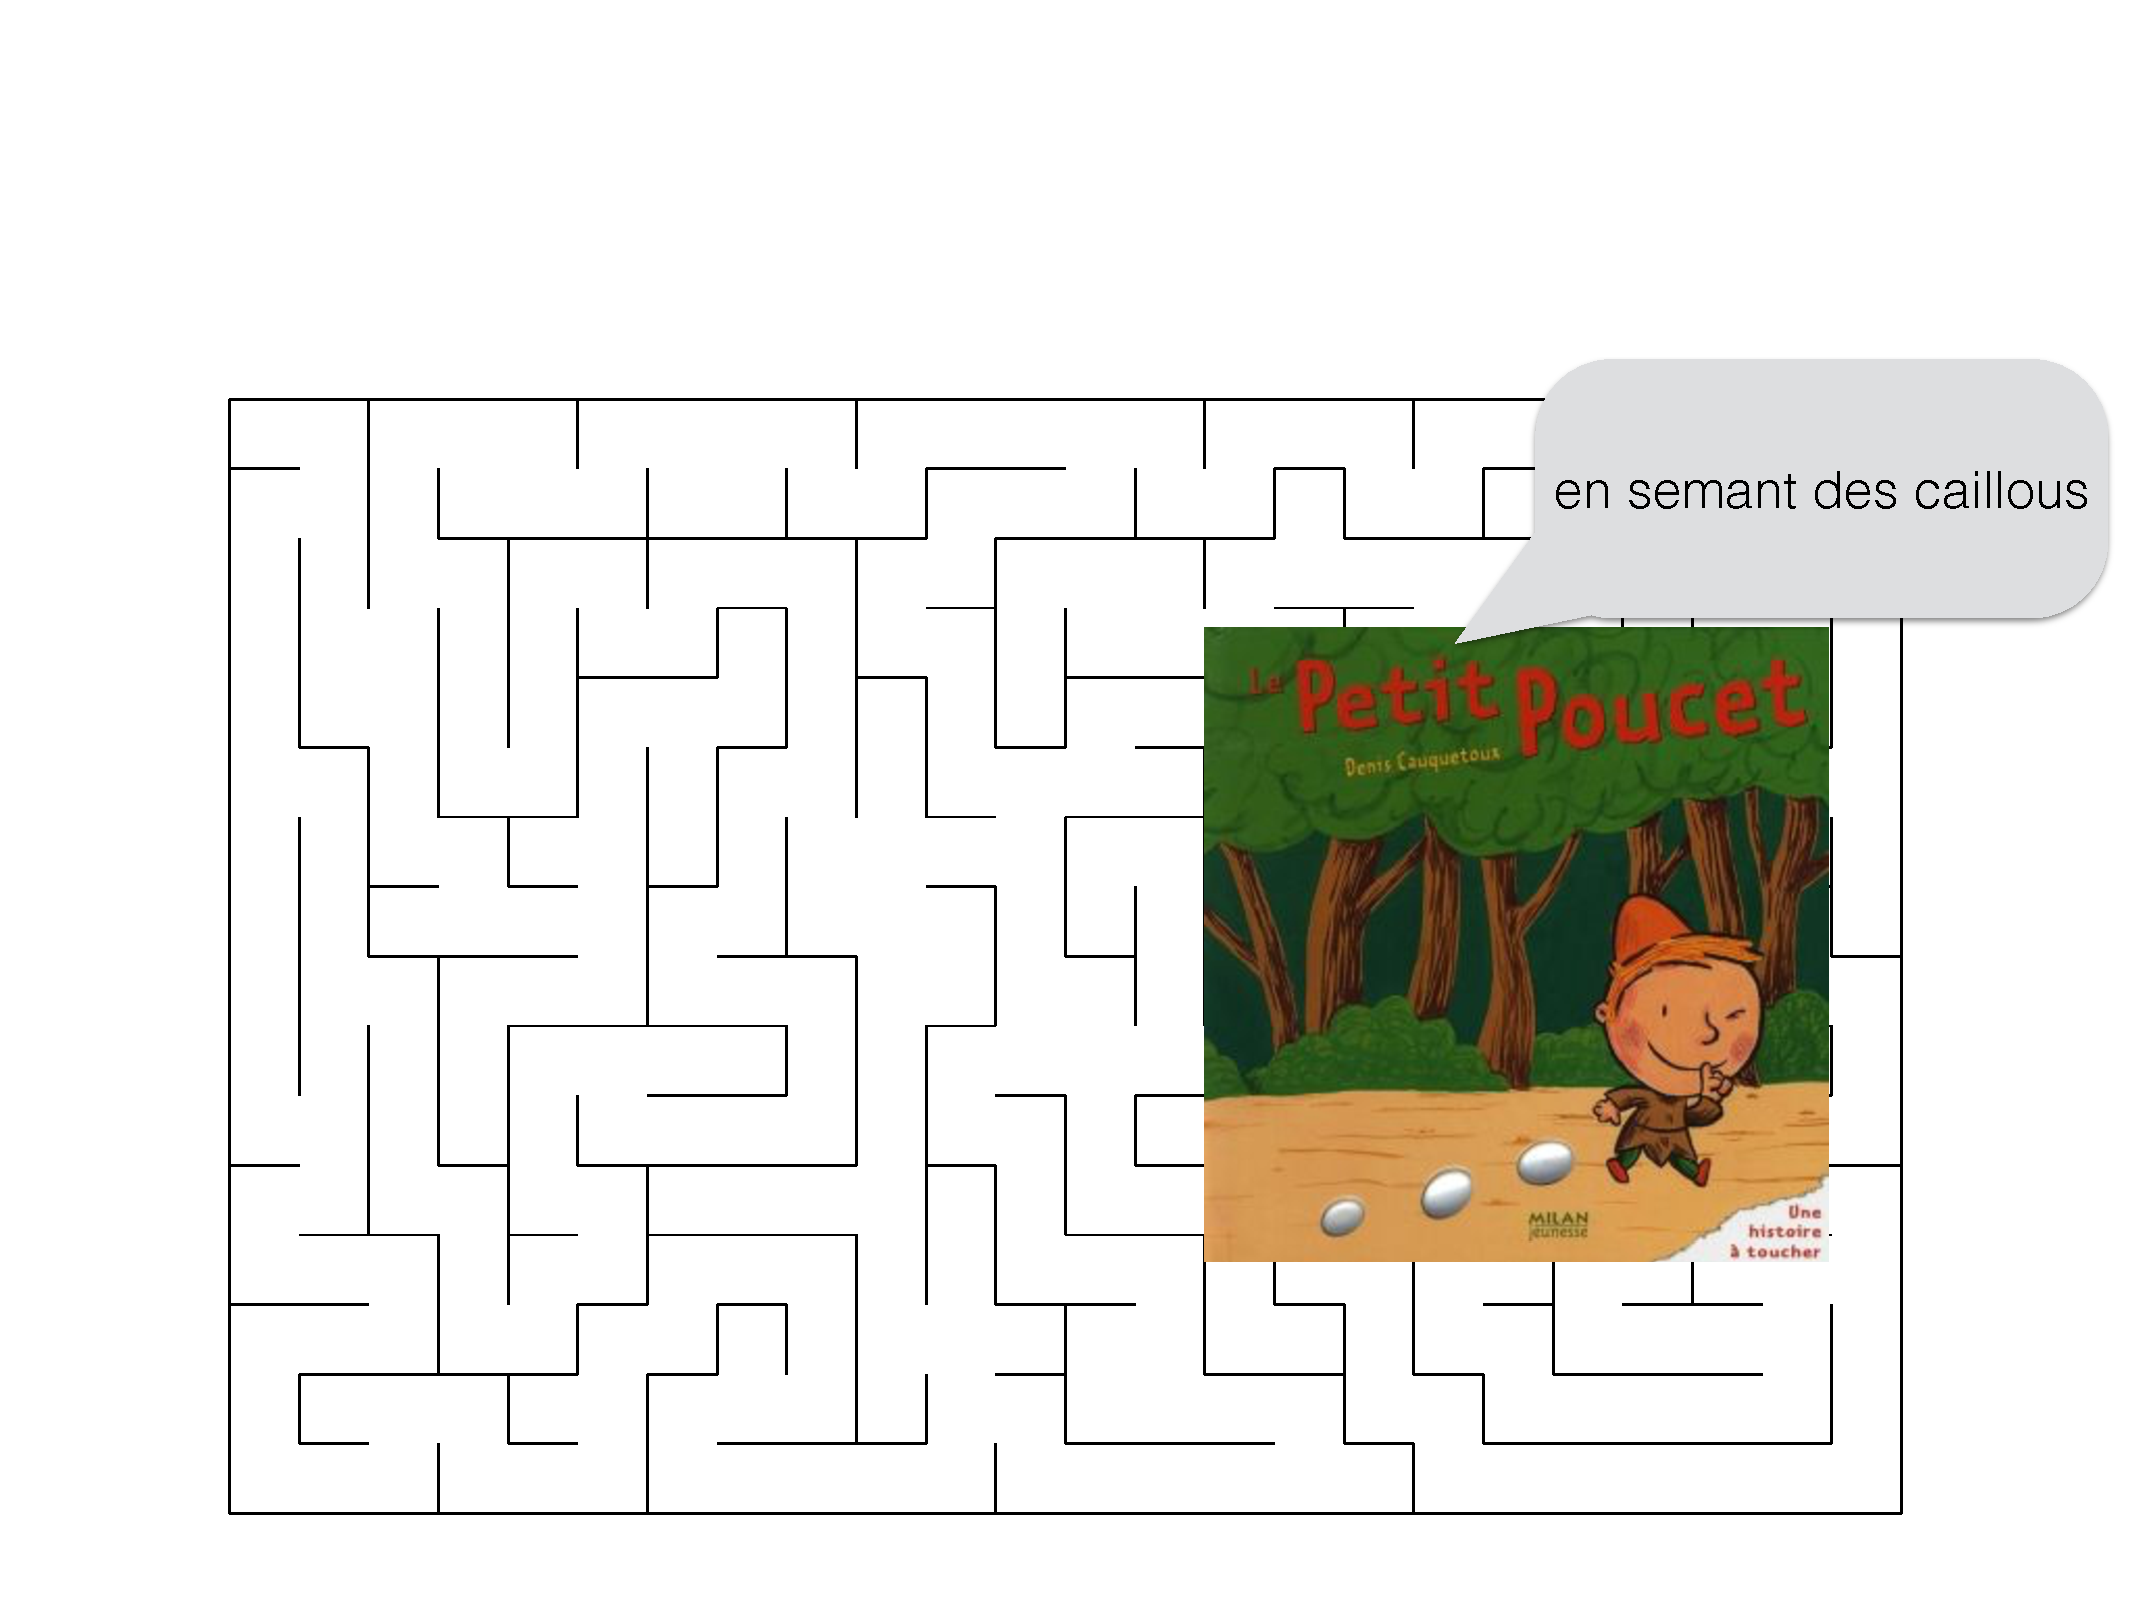
\includegraphics[width=.75\textwidth]{fig/labyrinthe-cailloux.pdf}
    \end{center}
\end{frame}

\begin{frame}{Comment ?}
    \begin{center}
        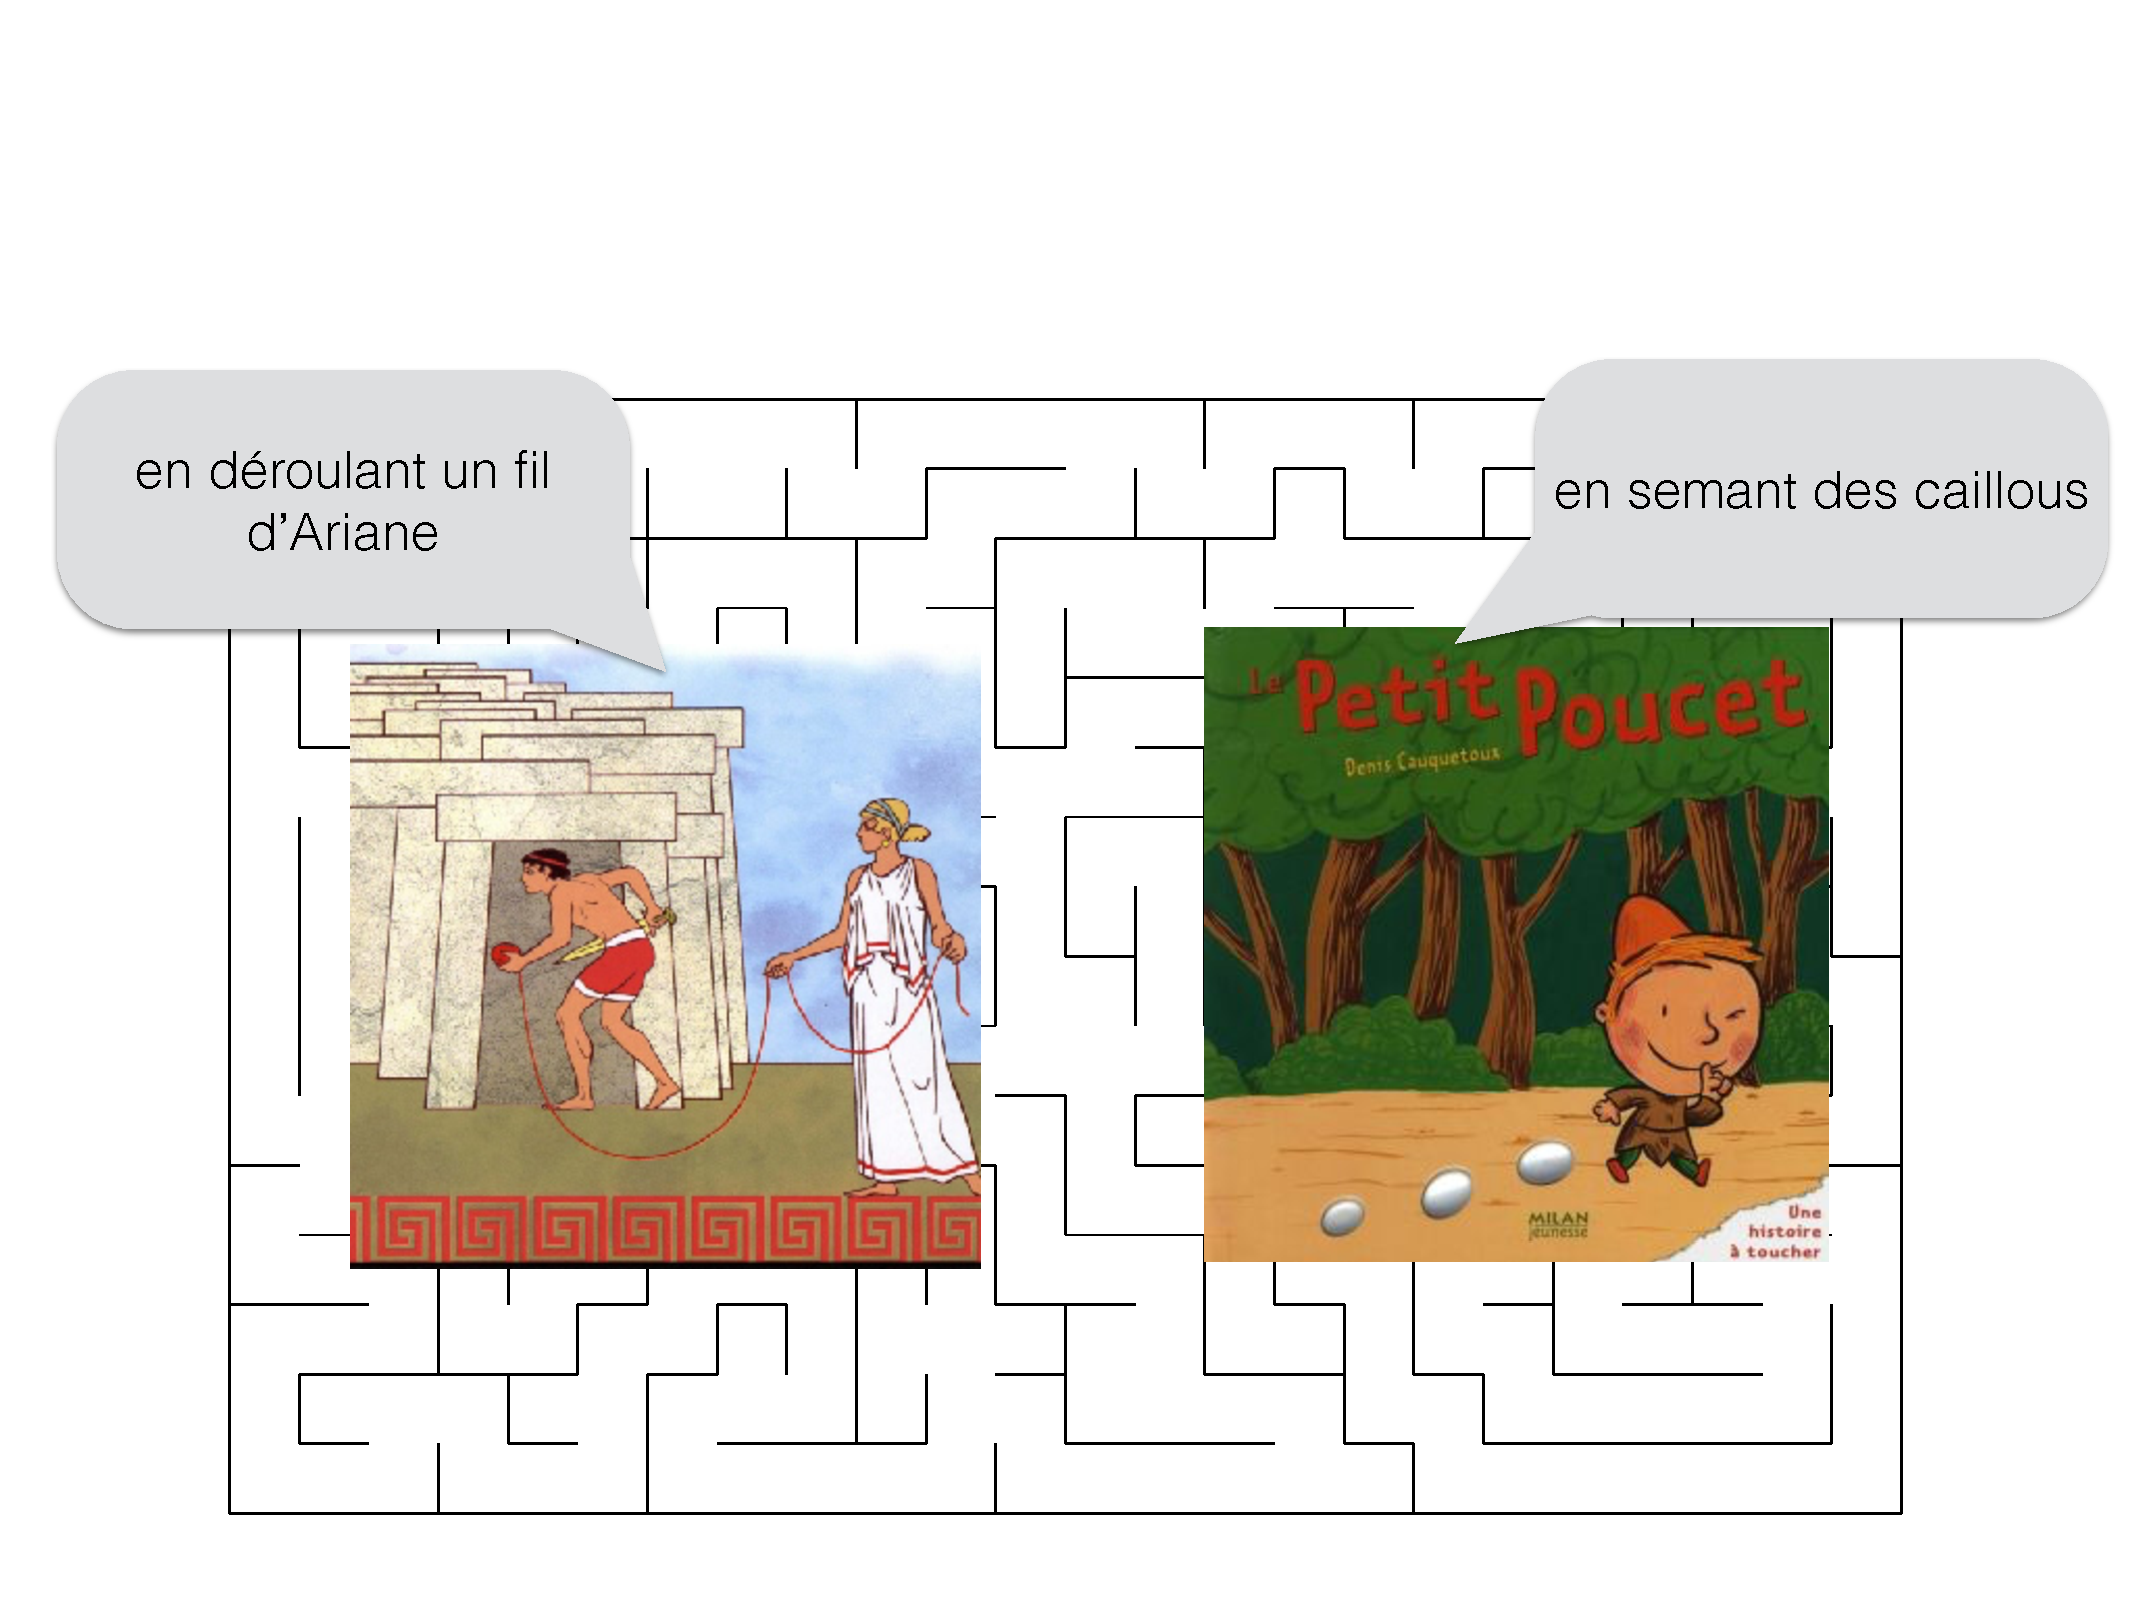
\includegraphics[width=.75\textwidth]{fig/labyrinthe-3.pdf}
    \end{center}
\end{frame}

\begin{frame}[fragile]
\frametitle{Parcours en profondeur}
    \begin{itemize}
        \item On utilise un tableau de booléens 
        \begin{itemize}
            \item \emph{vrai} si le sommet a été vu 
            \item \emph{faux} sinon 
        \end{itemize}
        \item on construit une fonction récursive \texttt{visite(i)} qui va explorer les sommets non vus à partir de $i$ ($i$ inclus)
    \end{itemize}
    
    % test
    \begin{algorithm}[H]
        \begin{algorithmic}[1]
            \Function{visite}{$i$ : sommet}
            \State vu[i] \gets true
            \For{$j \in Adj[i]$}
                \If{$vu[j] = false$}
                    \State visite(j)
                \EndIf
            \EndFor
            \EndFunction
         \end{algorithmic}
        \caption{Parcours en profondeur à partir d'un sommet}
        \label{alg:prof:visite}
        \end{algorithm}
\end{frame}



% ajouter la version avec les dates de visite ? pas sûr de l'intérêt ici...

\begin{frame}{Parcours en profondeur}
    \begin{itemize}
        \item Attention : l'algorithme n'est pas correct pour parcourir tout le graphe
        \item De fait, il ne fonctionne que si le graphe est connexe 
        \pause 
        \item On peut ajouter une boucle sur tous les sommets 
        \pause 
        \begin{algorithm}[H]
            \begin{algorithmic}[1]
                \State vu \gets [$false$,...,$false$]
                \For{$i \in S$}
                    \If{$vu[i] = false$}
                        \State visite(i)
                    \EndIf
                \EndFor
             \end{algorithmic}
            \caption{Parcours en profondeur}
            \label{alg:prof:alg}
            \end{algorithm}
        \pause 
        \item convention implicite : on parcourt les sommets et les adjacents en ordre croissant
    \end{itemize}
\end{frame}


\directlua{\detokenize{
    for i=0,6,1 do
        tex.sprint("\\begin{frame}{Exemple} \\input{genfig/pp-", i, ".tex} \\end{frame}")
    end
}}

\begin{frame}{Efficacité de l'algorithme}
    \begin{itemize}
        \item On marque $vu[i]$ une seule fois 
        \begin{itemize}
            \item Donc \texttt{visite(i)} termine toujours
            \item \texttt{visite(i)} n'est appelée qu'une seule fois par sommet
        \end{itemize}
        \item Le temps de calcul est dominé par les itérations de boucles
        \begin{itemize}
            \item La boucle principale s'exécute $n$ fois 
            \item La boucle secondaire s'exécute globalement $\sum_i | Adj[i] | = m$
        \end{itemize}
        \item La complexité pire cas est en $n+m$, donc linéaire
    \end{itemize}
\end{frame}

\begin{frame}{Forêts de parcours}
    \begin{itemize}
        \item Pendant un parcours en profondeur récursif, on peut créer une relation \emph{parent} qui mémorise pour chaque sommet $j$ 
        \begin{itemize}
            \item le sommet $i$ responsable de sa visite 
            \item $-1$ si le sommet $j$ est visité par la boucle principale 
        \end{itemize}
        \item Le graphe non-orienté associé à \emph{parent} (une arête entre $i$ et $j$ si $parent[i]=j$), forme une forêt de parcours 
    \end{itemize}
\end{frame}



\begin{frame}[fragile]
\frametitle{Algorithme}
    \begin{columns}
        \begin{column}{.5\textwidth}
            \begin{algorithmic}[1]
                \Function{visite}{$i$ : sommet}
                \State vu[i] \gets true
                \For{$j \in Adj[i]$}
                    \If{$vu[j] = false$}
                        \State \textcolor{blue}{parent[j] \gets i}
                        \State visite(j)
                    \EndIf
                \EndFor
                \EndFunction
            \end{algorithmic}
        \end{column}
        \begin{column}{.5\textwidth}
            \begin{algorithmic}[1]
                \State vu \gets [$false$,...,$false$]
                \State \textcolor{blue}{parent \gets [$-1$,...,$-1$]}
                \For{$i \in S$}
                    \If{$vu[i] = false$}
                    \State visite(i)
                    \EndIf
                \EndFor
                \end{algorithmic}            
        \end{column}
    \end{columns}    
\end{frame}


% ajouter un exemple sur les forets de parcours 
% cours David : 
%  un exemple jouet que je ne comprends pas 
%  un exemple de parcours sur un très grand graphe 

\begin{frame}{Exemples d'application}
    \begin{itemize}
        \item Les arbres (forêts) de parcours ont diverses applications
        \item Composantes connexes 
        \begin{itemize}
            \item Identification
            \item Parcours 
        \end{itemize}
        \item Graphe bipartis
    \end{itemize}
\end{frame}


\begin{frame}{Composantes connexes}
    \begin{itemize}
        \item Propriétés du parcours en profondeur
        \begin{itemize}
            \item \texttt{visite(i)} ne parcourt que les sommets accessibles depuis $i$ 
            \item elle parcourt tous ceux qui n'étaient pas marqués \texttt{vu} avant de démarrer la fonction 
        \end{itemize}
        \item Comptage du nombre de composantes connexes 
        \begin{itemize}
            \item Il suffit de rajouter un compteur dans la boucle principale 
            \item incrémenté à chaque appel à \texttt{visite(i)}
        \end{itemize}
    \end{itemize}
    \begin{center}
        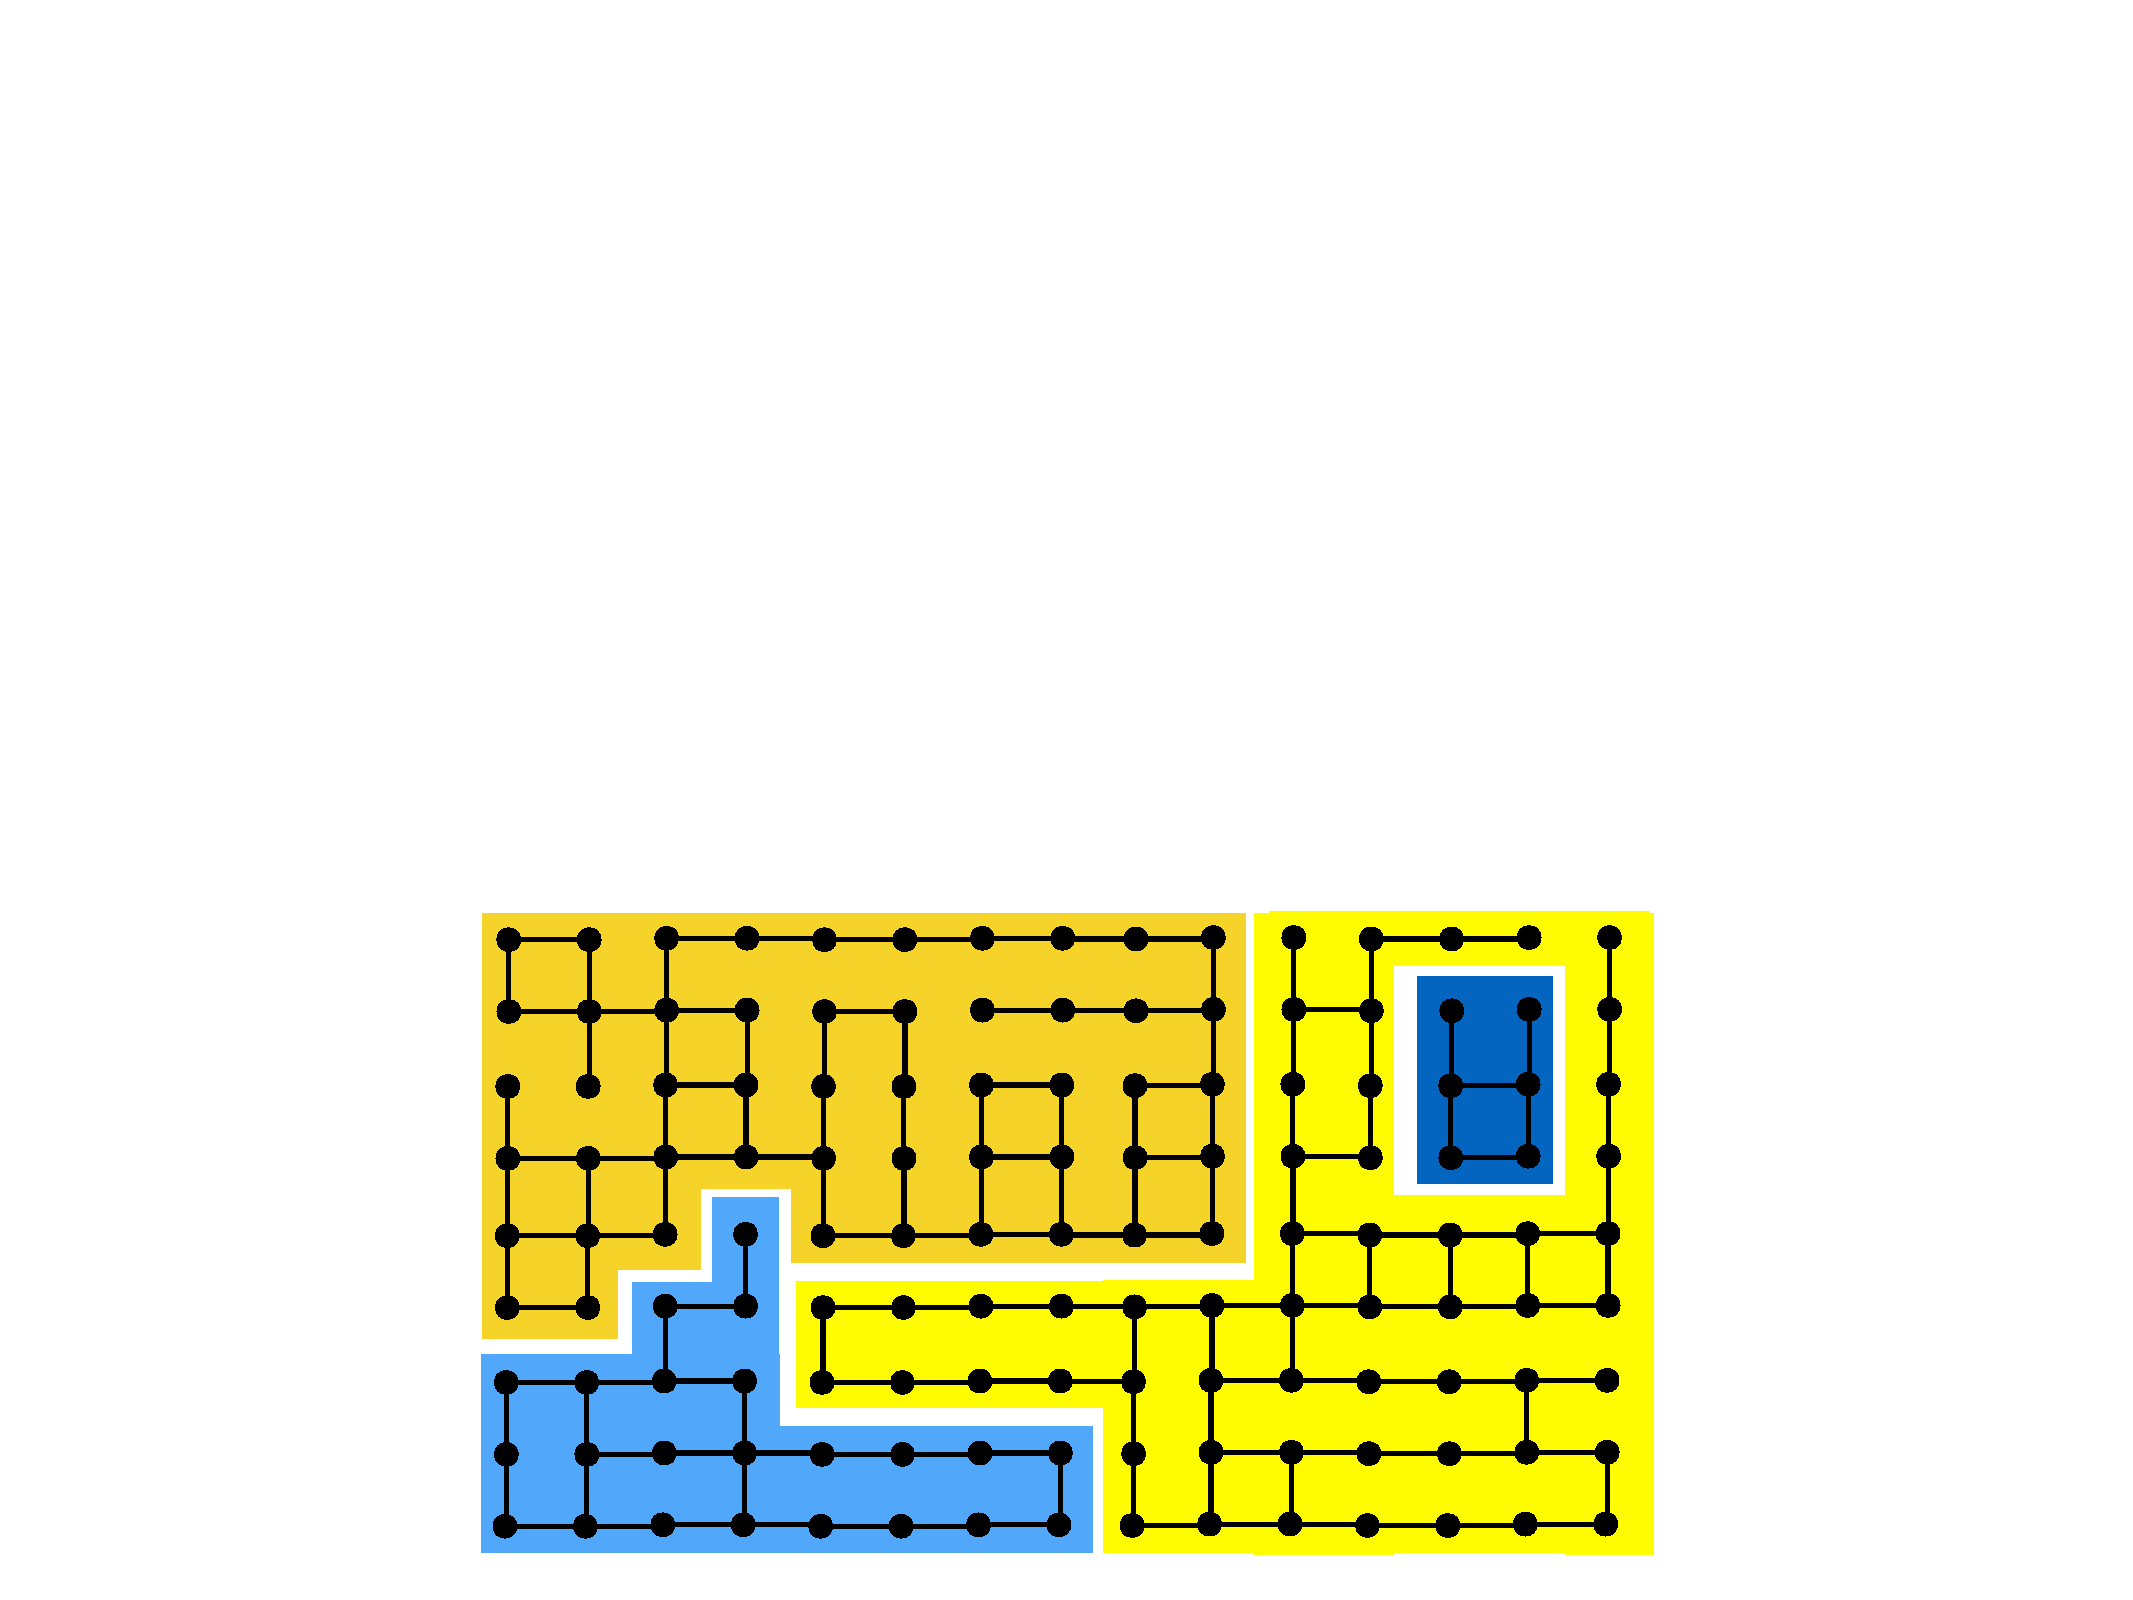
\includegraphics[width=.5\textwidth]{fig/cc.pdf}
    \end{center}
\end{frame}

\begin{frame}{Graphe biparti : plan de table}
    \begin{example}
        Pour un repas de famille, on doit réaliser un plan de table en tenant compte des inimitiés : les personnes qui ne s'aiment pas ne doivent pas se retrouver à la même table.        
    \end{example}
    \begin{center}
        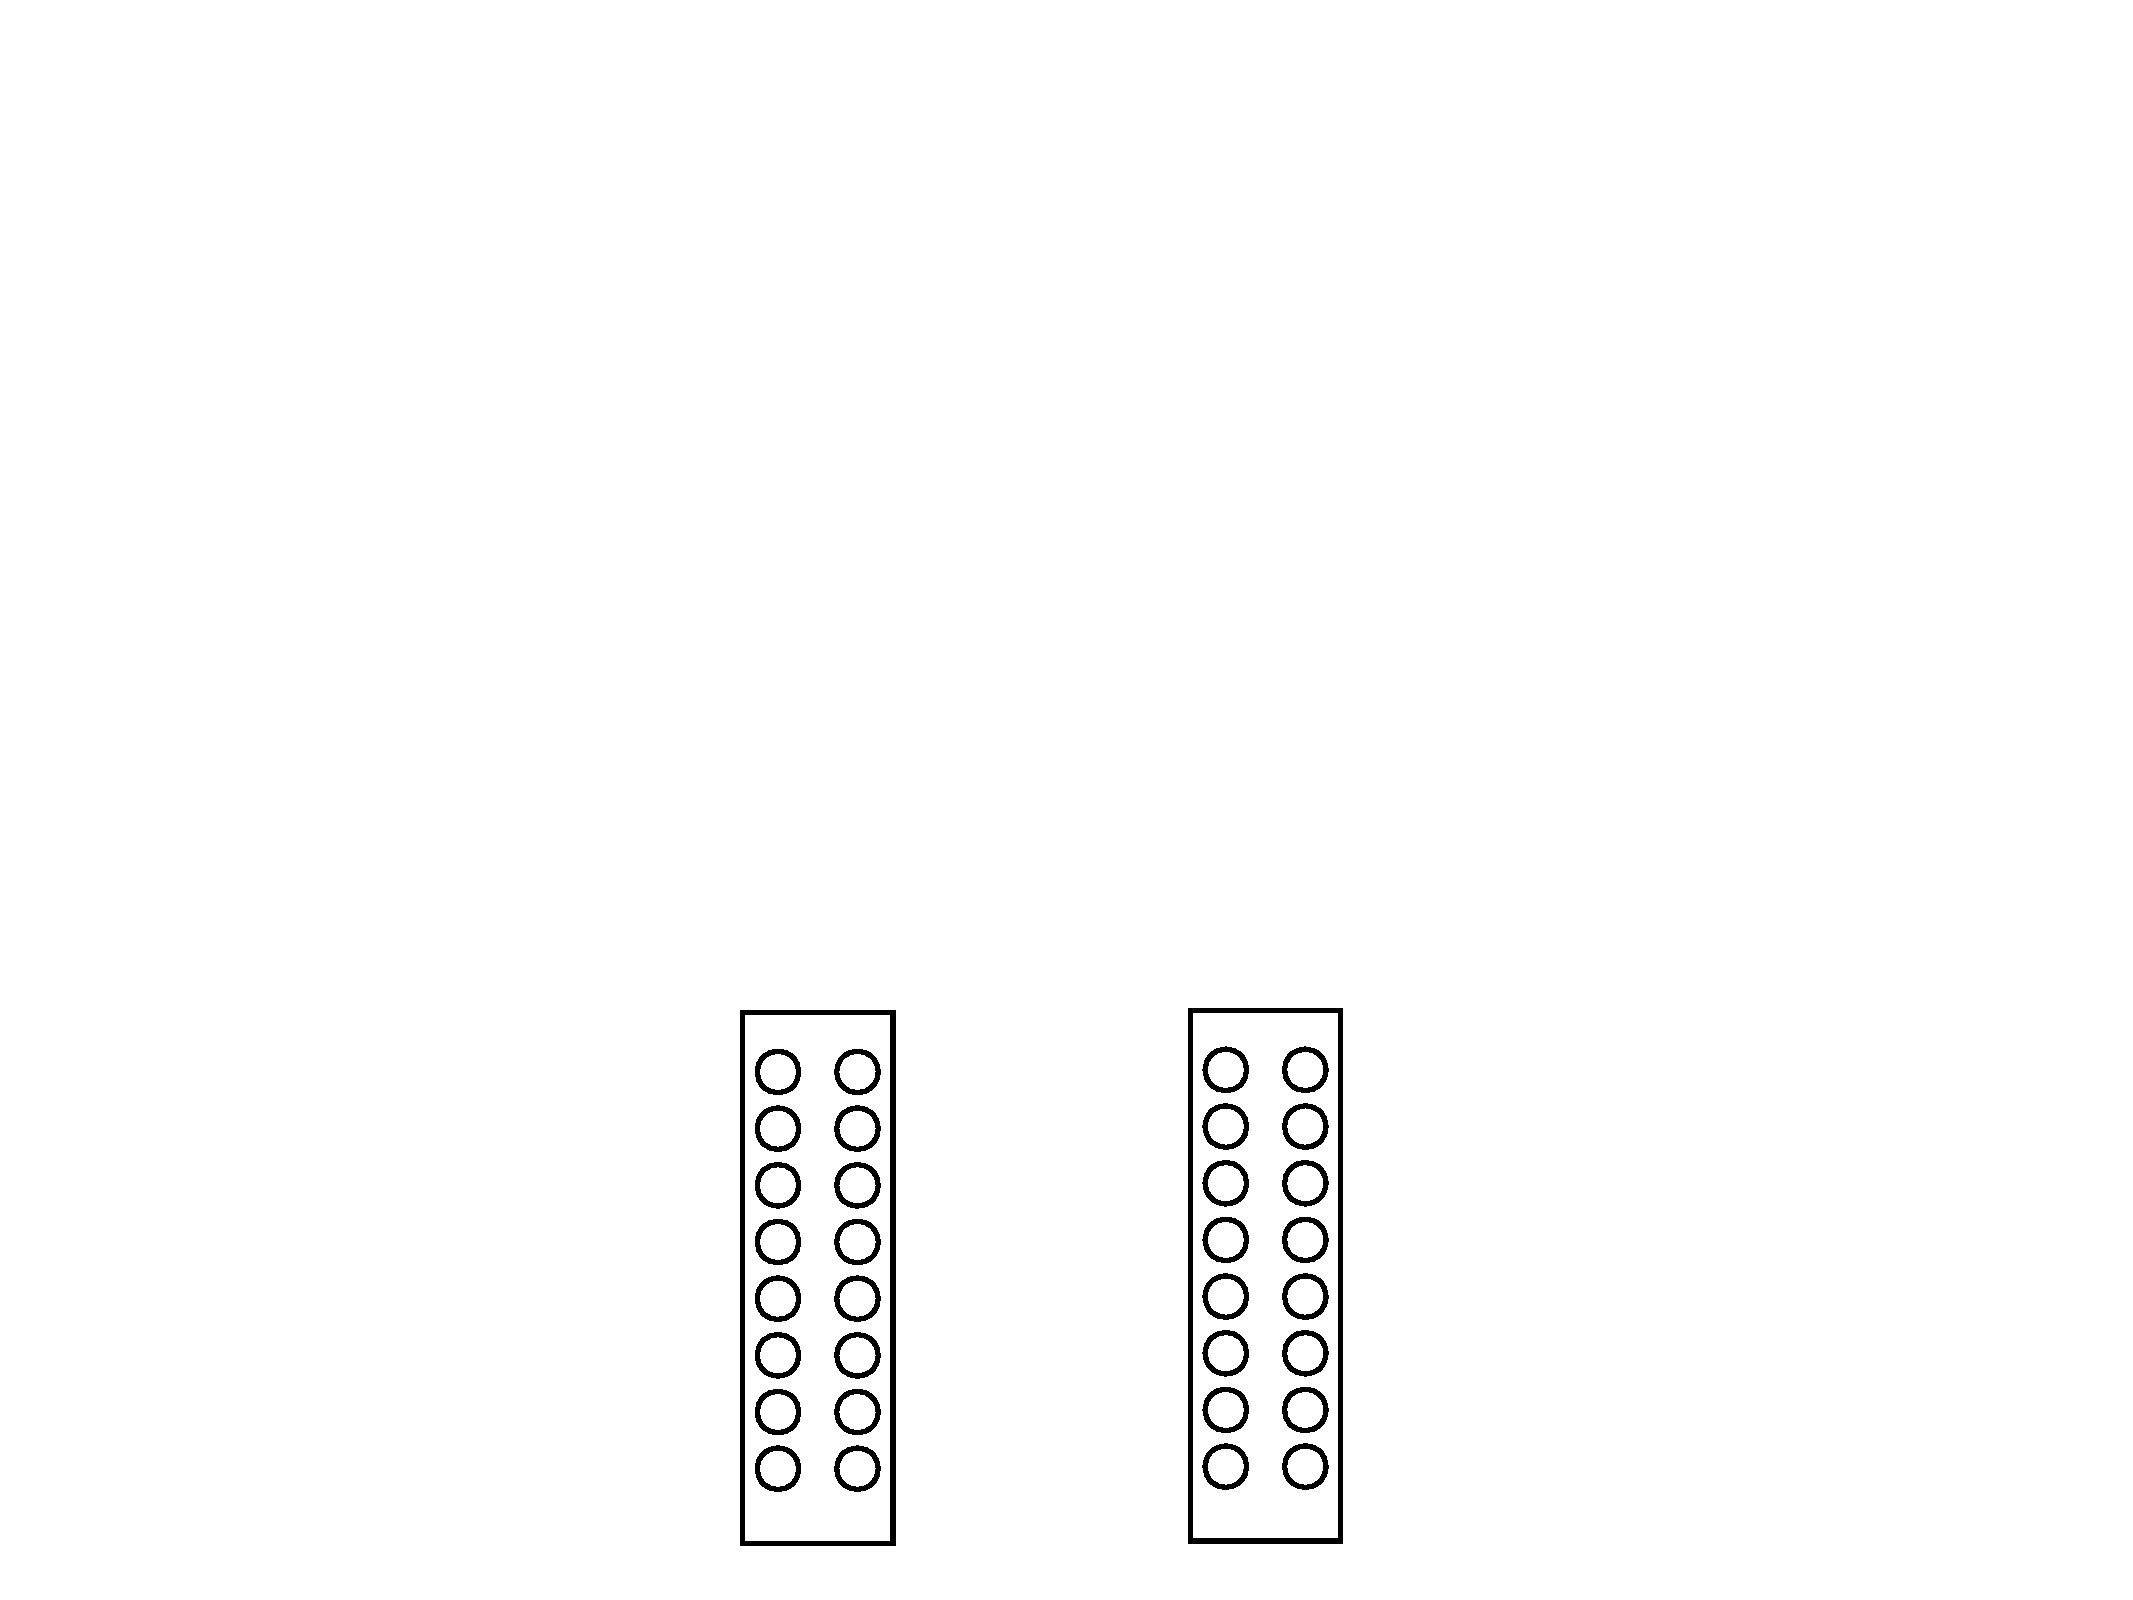
\includegraphics[width=.2\textwidth]{fig/plandetable.pdf}
    \end{center}
    \begin{definition}
        Un graphe non orienté est \emph{biparti} si l'ensemble des sommets peut être séparé en deux ensembles disjoints $S_1$ et $S_2$ tel que chaque arête du graphe relie un sommet de $S_1$ à un sommet de $S_2$ 
    \end{definition}
\end{frame}

\begin{frame}{Exemple}
    \begin{center}
    \begin{tikzpicture}
        \tikzstyle{sommet}=[circle,draw,fill=black]
        \node[sommet] (1) at (1,0) {};
        \node[sommet] (2) at (1,-1) {};
        \node[sommet] (3) at (1,-2) {};
        \node[sommet] (4) at (1,-3) {};
        \node[sommet] (5) at (2,0) {};
        \node[sommet] (6) at (2,-1) {};
        \node[sommet] (7) at (2,-2) {};
        \node[sommet] (8) at (2,-3) {};
        \node[sommet] (9) at (3,0) {};
        \node[sommet] (10) at (3,-1) {};
        \node[sommet] (11) at (3,-2) {};
        \node[sommet] (12) at (3,-3) {};
        \node[sommet] (13) at (4,0) {};
        \node[sommet] (14) at (4,-1) {};
        \node[sommet] (15) at (4,-2) {};
        \node[sommet] (16) at (4,-3) {};
        \node[sommet] (17) at (5,0) {};
        \node[sommet] (18) at (5,-1) {};
        \node[sommet] (19) at (5,-2) {};
        \node[sommet] (20) at (5,-3) {};
        \node[sommet] (21) at (6,0) {};
        \node[sommet] (22) at (6,-1) {};
        \node[sommet] (23) at (6,-2) {};
        \node[sommet] (24) at (6,-3) {};
        \draw (1) -- (2) -- (3) -- (4);
        \draw (6) -- (7) -- (8);
        \draw (9) -- (10) -- (11);
        \draw (13) -- (14);
        \draw (15) -- (16);
        \draw (17) -- (18) -- (19);
        \draw (21) -- (22) -- (23);
        \draw (2) -- (6) -- (10) -- (14) -- (18);
        \draw (3) -- (7) -- (11);
        \draw (19) -- (23);
        \draw (4) -- (8);
        \draw (12) -- (16);
        \draw (20) -- (24); 
    \end{tikzpicture}
\end{center}
\end{frame}

\begin{frame}{Exemple}
    \begin{center}
    \begin{tikzpicture}
    \tikzstyle{sommetA}=[circle,draw,fill=blue]
    \tikzstyle{sommetB}=[circle,draw,fill=red]
    \node[sommetA] (1) at (1,0) {};
    \node[sommetB] (2) at (1,-1) {};
    \node[sommetA] (3) at (1,-2) {};
    \node[sommetB] (4) at (1,-3) {};
    \node[sommetA] (5) at (2,0) {};
    \node[sommetA] (6) at (2,-1) {};
    \node[sommetB] (7) at (2,-2) {};
    \node[sommetA] (8) at (2,-3) {};
    \node[sommetA] (9) at (3,0) {};
    \node[sommetB] (10) at (3,-1) {};
    \node[sommetA] (11) at (3,-2) {};
    \node[sommetA] (12) at (3,-3) {};
    \node[sommetB] (13) at (4,0) {};
    \node[sommetA] (14) at (4,-1) {};
    \node[sommetA] (15) at (4,-2) {};
    \node[sommetB] (16) at (4,-3) {};
    \node[sommetA] (17) at (5,0) {};
    \node[sommetB] (18) at (5,-1) {};
    \node[sommetA] (19) at (5,-2) {};
    \node[sommetB] (20) at (5,-3) {};
    \node[sommetB] (21) at (6,0) {};
    \node[sommetA] (22) at (6,-1) {};
    \node[sommetB] (23) at (6,-2) {};
    \node[sommetA] (24) at (6,-3) {};
    \draw (1) -- (2) -- (3) -- (4);
    \draw (6) -- (7) -- (8);
    \draw (9) -- (10) -- (11);
    \draw (13) -- (14);
    \draw (15) -- (16);
    \draw (17) -- (18) -- (19);
    \draw (21) -- (22) -- (23);
    \draw (2) -- (6) -- (10) -- (14) -- (18);
    \draw (3) -- (7) -- (11);
    \draw (19) -- (23);
    \draw (4) -- (8);
    \draw (12) -- (16);
    \draw (20) -- (24); 
\end{tikzpicture}
\end{center}
\end{frame}

\begin{frame}[fragile]
\frametitle{Algorithme : principe}

\begin{itemize}
    \item Pendant un parcours en profondeur, on associe une couleur (0 ou 1) à chaque sommet en s'assurant que deux sommets adjacents n'ont pas la même couleur 
    \item Si l'algorithme termine sans erreur, on a examiné chaque arête et attribué des couleurs cohérentes à chaque sommet : le graphe est biparti 
    \item Sinon, le coloriage est impossible et l'algorithme s'arrête avant la fin 
\end{itemize}
\end{frame}

    \begin{frame}[fragile]
        \frametitle{Algorithme}
            \begin{columns}
                \begin{column}{.55\textwidth}
                    \begin{algorithmic}
                    \Function{visite}{$i$ : sommet,$c$ : int}
                    \State vu[i] \gets true
                    \State couleur[i] \gets $c$
                    \For{$j \in Adj[i]$}
                        \If{$vu[j] = false$}
                            \State visite(j,1-$c$)
                        \ElsIf{couleur[j] = $c$} 
                                \State STOP("pas biparti")
                        \EndIf
                    \EndFor
                    \EndFunction
                                    \end{algorithmic}
                \end{column}
                \begin{column}{.45\textwidth}
                    \begin{algorithmic}
                        \State vu \gets [$false$,...,$false$]
                        \State couleur \gets $[-1,...,-1]$
                        \For{$i \in S$}
                            \If{$vu[i] = false$}
                                \State visite(i)
                            \EndIf
                        \EndFor
                    \end{algorithmic}            
                \end{column}
            \end{columns}    
        \end{frame}
        
\begin{frame}{k-coloration}
\begin{definition}
    Un graphe non-orienté est \emph{$k$-coloriable} si on peut colorier chaque sommet avec une couleur comprise entre $1$ et $k$, de telle façon que deux sommets adjacents aient des couleurs distinctes
\end{definition}
\begin{itemize}
    \item Remarques 
    \begin{itemize}
        \item Un graphe biparti est un graphe $2$-coloriable 
        \item L'algorithme de $2$-coloration vu précédemment est linéaire, ce n'est pas généralisable malheureusement
        \item De fait, pour $k>2$, le problème de déterminer si un graphe est $k$-coloriable est NP-complet  
    \end{itemize}
\end{itemize}
\end{frame}

% parcours en profondeur (version non récursive) 

\begin{frame}{Dérécursification}

\begin{itemize}
    \item Tout programme récursif peut être transformé en un programme équivalent non récursif, en s'aidant d'une \emph{pile} 
    \begin{itemize}
        \item cela peut avoir un intérêt pour l'efficacité (peu probable)
        \item certains compilateurs savent le faire automatiquement (HS ici) 
        \item dans certains cas, c'est plus facile à comprendre 
    \end{itemize}
\end{itemize}
\end{frame}

\begin{frame}[fragile]
    \frametitle{Algorithme de parcours en profondeur itératif}
        \begin{columns}
            \begin{column}{.55\textwidth}
                \begin{algorithmic}
                    \Function{visite}{$i$ : sommet}
                    \State P \gets empty() 
                    \State vi[i] \ gets true 
                    \State push(P,i) 
                    \While{!empty(P)}
                        \State k \gets pop(P)
                        \For{$j \in Adj[k]$}
                            \If{!vu[j]} 
                            \State vu[k] \gets true 
                            \State push(P,j
                            \EndIf
                        \EndFor
                    \EndWhile
                    \EndFunction
                \end{algorithmic}
            \end{column}
            \begin{column}{.45\textwidth}
                \begin{algorithmic}
                    \State vu \gets [$false$,...,$false$]
                    \For{$i \in S$}
                        \If{$vu[i] = false$}
                            \State visite(i)
                        \EndIf
                    \EndFor
                \end{algorithmic}            
            \end{column}
        \end{columns}    
    \end{frame}



% Algorithmes de plus courts chemins 
\section{Algorithmes de plus courts chemins}
% algorithmes de plus courts chemins 

\begin{frame}{Graphes pondérés}

\begin{definition}
    Un graphe \emph{non-orienté pondéré} est un graphe non-orienté muni d'une fonction de pondération qui associe une valeur réelle à chaque arête. 
\end{definition}

\begin{definition}
    Un graphe \emph{orienté pondéré} est un graphe orienté muni d'une fonction de pondération qui associe une valeur réelle à chaque arc. 
\end{definition}

\end{frame}

\begin{frame}{Exemple : graphe non-orienté pondéré}
    \begin{center}
        \begin{tikzpicture}
\clip (0,0) rectangle (6,6);
\Vertex[x=0.450,y=5.550,size=0.8,opacity=0.5,label=1]{0}
\Vertex[x=0.450,y=3.000,size=0.8,opacity=0.5,label=2]{1}
\Vertex[x=3.000,y=3.000,size=0.8,opacity=0.5,label=3]{2}
\Vertex[x=3.000,y=5.550,size=0.8,opacity=0.5,label=4]{3}
\Vertex[x=5.550,y=5.550,size=0.8,opacity=0.5,label=5]{4}
\Vertex[x=5.550,y=3.000,size=0.8,opacity=0.5,label=6]{5}
\Vertex[x=5.550,y=0.450,size=0.8,opacity=0.5,label=7]{6}
\Vertex[x=3.000,y=0.450,size=0.8,opacity=0.5,label=8]{7}
\Vertex[x=0.450,y=0.450,size=0.8,opacity=0.5,label=9]{8}
\Edge[,lw=2.0,bend=-8.531,label=5](0)(1)
\Edge[,lw=2.0,bend=-8.531,label=2](0)(3)
\Edge[,lw=2.0,bend=-8.531,label=-2](1)(3)
\Edge[,lw=2.0,bend=-8.531,label=4](2)(8)
\Edge[,lw=2.0,bend=-8.531,label=1](4)(5)
\Edge[,lw=2.0,bend=-8.531,label=3](5)(6)
\Edge[,lw=2.0,bend=-8.531,label=0](6)(7)
\end{tikzpicture}

    \end{center}
    \end{frame}

% TODO exemple de graphe orienté avec pondération ?

\begin{frame}{Applications}
    \begin{itemize}
        \item Calcul de plus courts chemins 
        \begin{itemize}
            \item Distances entre villes
        \end{itemize}
        \item Arbres couvrants minimaux 
        \item Contraintes entre tâches 
    \end{itemize}
\end{frame}

\begin{frame}{Arbre couvrant}
    \begin{definition}
        Dans un graphe $G$ non orienté (pondéré ou non) connexe, un arbre couvrant est un sous-graphe connexe acyclique (arbre) incluant tous les sommets de $G$
    \end{definition}


\end{frame}

% TODO ajouter définition d'un sous-graphe 


\begin{frame}{Exemple : arbre couvrant}
    \begin{center}
        \begin{tikzpicture}
\clip (0,0) rectangle (6,6);
\Vertex[x=0.450,y=5.550,size=0.8,opacity=0.5,label=1]{0}
\Vertex[x=0.450,y=3.000,size=0.8,opacity=0.5,label=2]{1}
\Vertex[x=3.000,y=3.000,size=0.8,opacity=0.5,label=3]{2}
\Vertex[x=3.000,y=5.550,size=0.8,opacity=0.5,label=4]{3}
\Vertex[x=5.550,y=5.550,size=0.8,opacity=0.5,label=5]{4}
\Vertex[x=5.550,y=3.000,size=0.8,opacity=0.5,label=6]{5}
\Vertex[x=5.550,y=0.450,size=0.8,opacity=0.5,label=7]{6}
\Vertex[x=3.000,y=0.450,size=0.8,opacity=0.5,label=8]{7}
\Vertex[x=0.450,y=0.450,size=0.8,opacity=0.5,label=9]{8}
\Edge[,lw=2.0,bend=-8.531](0)(1)
\Edge[,lw=4.0,bend=-8.531](0)(3)
\Edge[,lw=4.0,bend=-8.531,](1)(3)
\Edge[,lw=4.0,bend=-8.531](2)(8)
\Edge[,lw=4.0,bend=-8.531](4)(5)
\Edge[,lw=4.0,bend=-8.531](5)(6)
\Edge[,lw=4.0,bend=-8.531](6)(7)
\Edge[,lw=4.0,bend=-8.531](3)(4)
\Edge[,lw=4.0,bend=-8.531](2)(6)
\Edge[,lw=2.0,bend=-8.531](2)(1)
\end{tikzpicture}

    \end{center}
    \end{frame}

    \begin{frame}{Contre-exemple : arbre non couvrant}
        \begin{center}
            \begin{tikzpicture}
\clip (0,0) rectangle (6,6);
\Vertex[x=0.450,y=5.550,size=0.8,opacity=0.5,label=1]{0}
\Vertex[x=0.450,y=3.000,size=0.8,opacity=0.5,label=2]{1}
\Vertex[x=3.000,y=3.000,size=0.8,opacity=0.5,label=3]{2}
\Vertex[x=3.000,y=5.550,size=0.8,opacity=0.5,label=4]{3}
\Vertex[x=5.550,y=5.550,size=0.8,opacity=0.5,label=5]{4}
\Vertex[x=5.550,y=3.000,size=0.8,opacity=0.5,label=6]{5}
\Vertex[x=5.550,y=0.450,size=0.8,opacity=0.5,label=7]{6}
\Vertex[x=3.000,y=0.450,size=0.8,opacity=0.5,label=8]{7}
\Vertex[x=0.450,y=0.450,size=0.8,opacity=0.5,label=9]{8}
\Edge[,lw=2.0,bend=-8.531](0)(1)
\Edge[,lw=4.0,bend=-8.531](0)(3)
\Edge[,lw=4.0,bend=-8.531,](1)(3)
\Edge[,lw=4.0,bend=-8.531](2)(8)
\Edge[,lw=2.0,bend=-8.531](4)(5)
\Edge[,lw=4.0,bend=-8.531](5)(6)
\Edge[,lw=4.0,bend=-8.531](6)(7)
\Edge[,lw=4.0,bend=-8.531](3)(4)
\Edge[,lw=4.0,bend=-8.531](2)(6)
\Edge[,lw=2.0,bend=-8.531](2)(1)
\end{tikzpicture}

        \end{center}
        \end{frame}
    
\begin{frame}{Construction d'un arbre couvrant}
\begin{itemize}
    \item Connaissez-vous un algorithme capable de construire un arbre couvrant ?
    \pause \item Oui !
    \pause \item Tous les algorithmes de parcours que nous avons vus jusqu'ici 
    \pause \item Pour de bonnes raisons applicatives, on va chercher à construire un arbre couvrant \emph{minimal} 
    \pause \item Est-on obligés de parcourir l'ensemble des arbres couvrants pour trouver un arbre de coût minimal ?
\end{itemize}
    
\end{frame}

\begin{frame}{Applications}
    \begin{itemize}
        \item Minimiser la longueur de câble nécessaire pour connecter un réseau 
        \item Heuristique dans certains problèmes d'optimisation
        \begin{itemize}
            \item problème du voyageur de commerce
        \end{itemize}
    \end{itemize}
\end{frame}

\begin{frame}{Arbre couvrant minimal}
    \begin{definition}
        Dans un graphe non orienté pondéré et connexe, un arbre couvrant minimal est un arbre couvrant dont la somme des arêtes est minimale
    \end{definition}

    \begin{itemize}
        \item Remarque : si le graphe n'est pas pondéré, on considère des arêtes de poids identique 
    \end{itemize}
\end{frame}

\begin{frame}{Exemple 1 : arbre couvrant minimal (non pondéré)}
    \begin{center}
        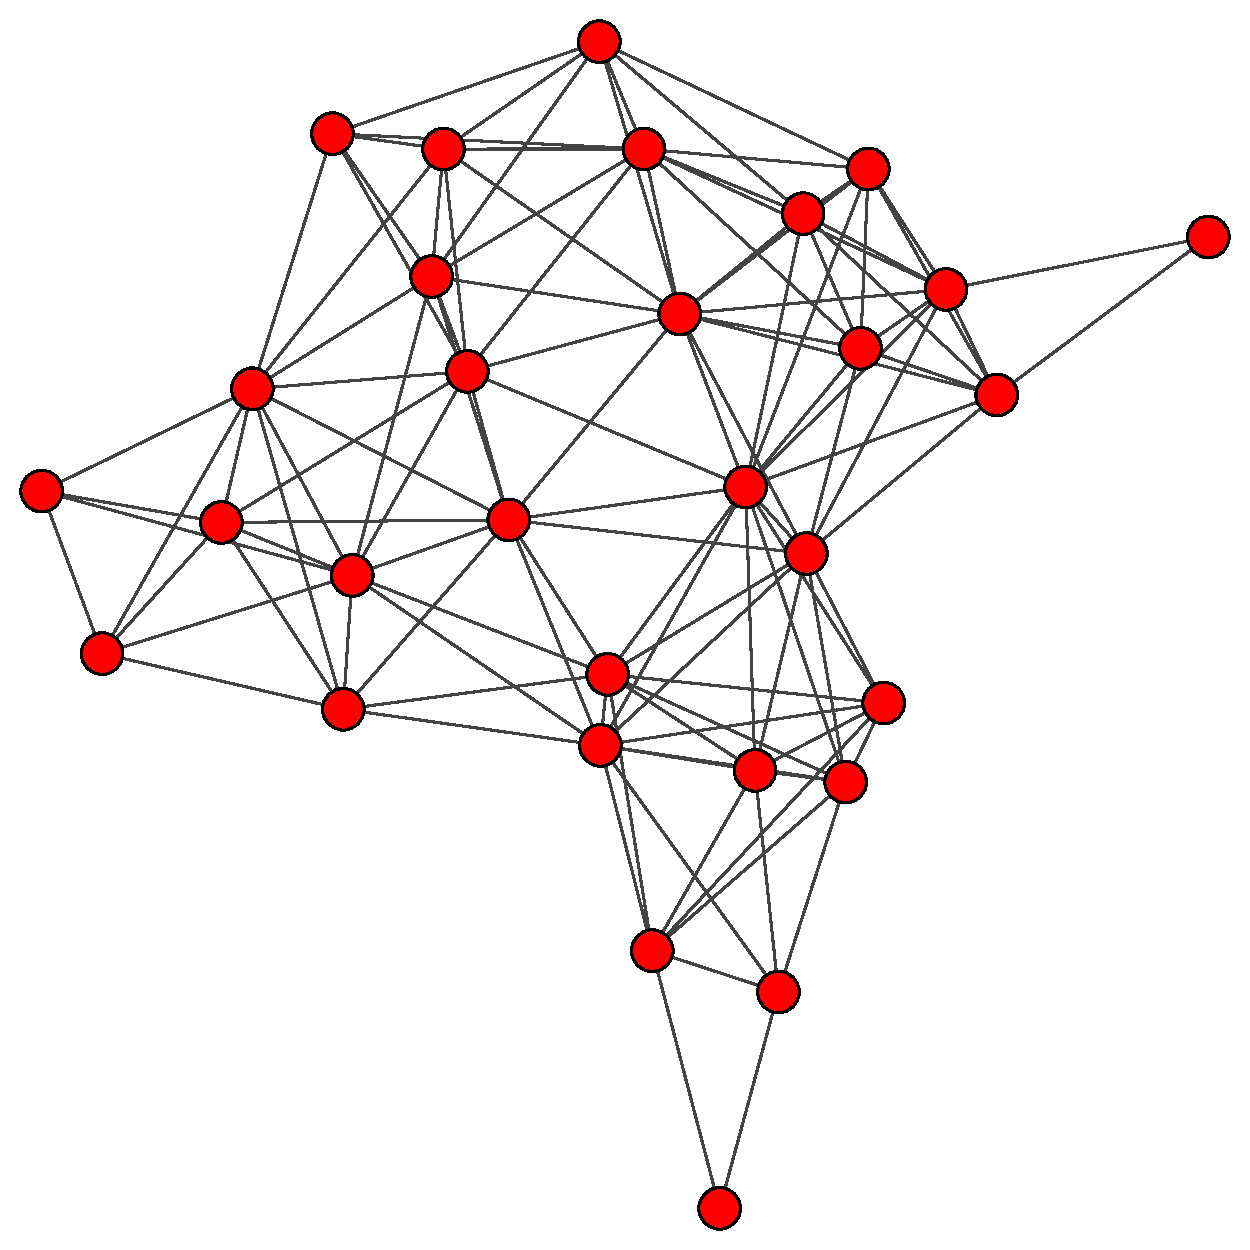
\includegraphics[height=.8\textheight]{fig/mst-0.pdf}
    \end{center}
\end{frame}
\begin{frame}{Exemple 1 : arbre couvrant minimal (non pondéré)}
    \begin{center}
        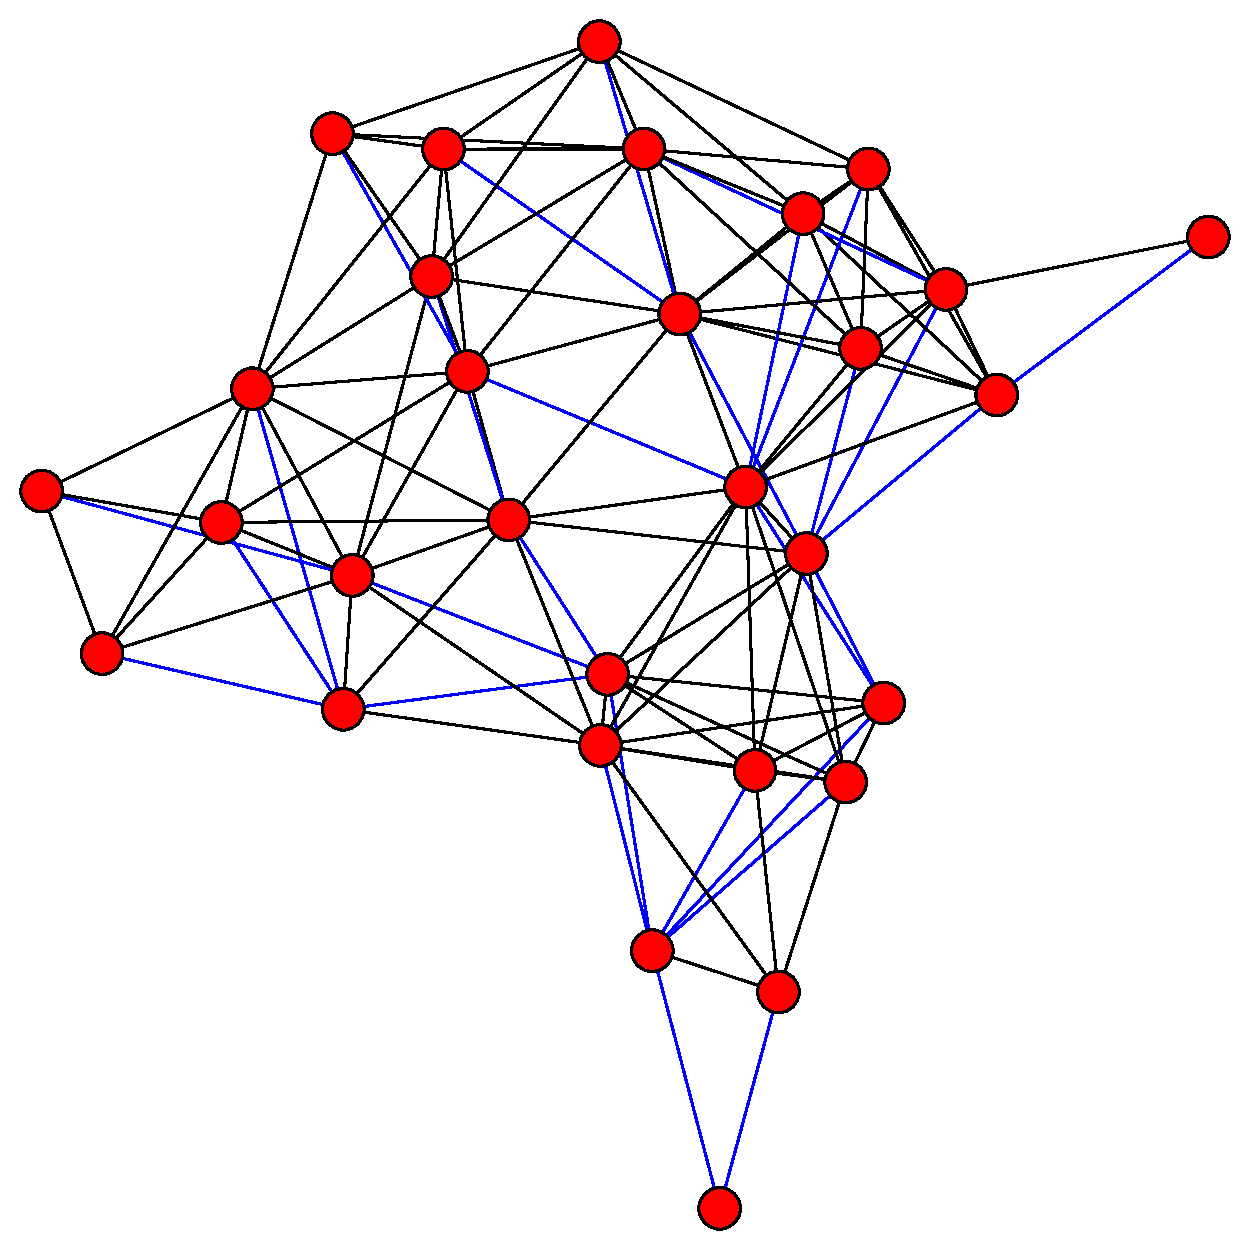
\includegraphics[height=.8\textheight]{fig/mst-1.pdf}
    \end{center}
\end{frame}
\begin{frame}{Exemple 1 : arbre couvrant minimal (non pondéré)}
    \begin{center}
        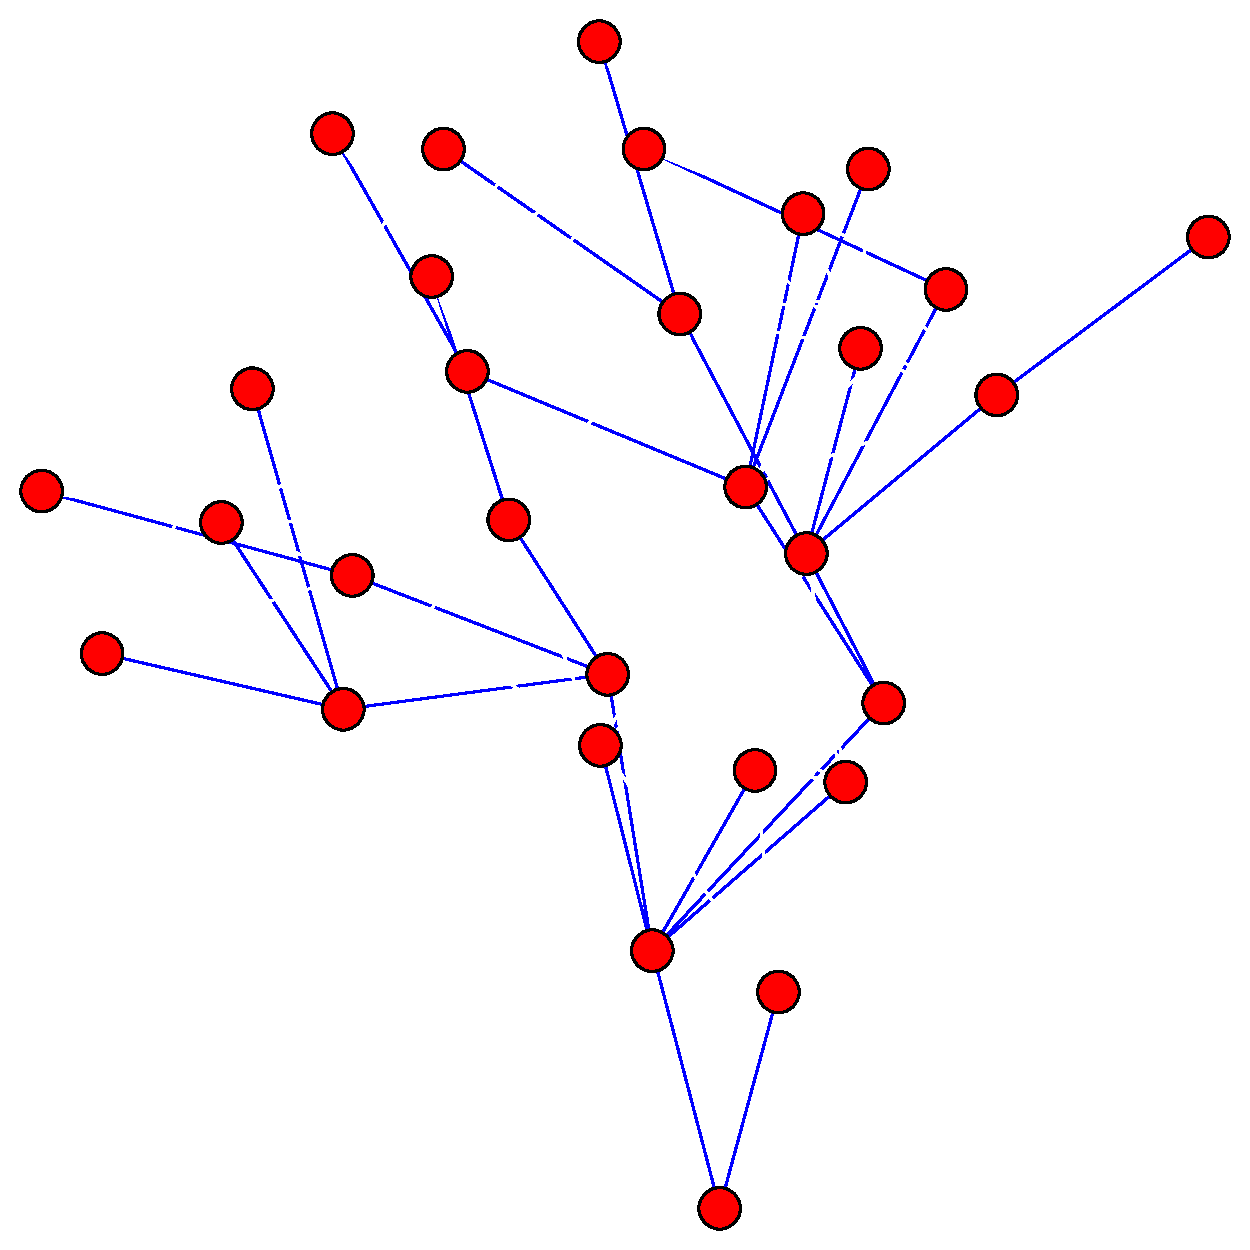
\includegraphics[height=.8\textheight]{fig/mst-2.pdf}
    \end{center}
\end{frame}

\begin{frame}{Exemple 2 : arbre couvrant minimal (pondéré)}
    \begin{center}
        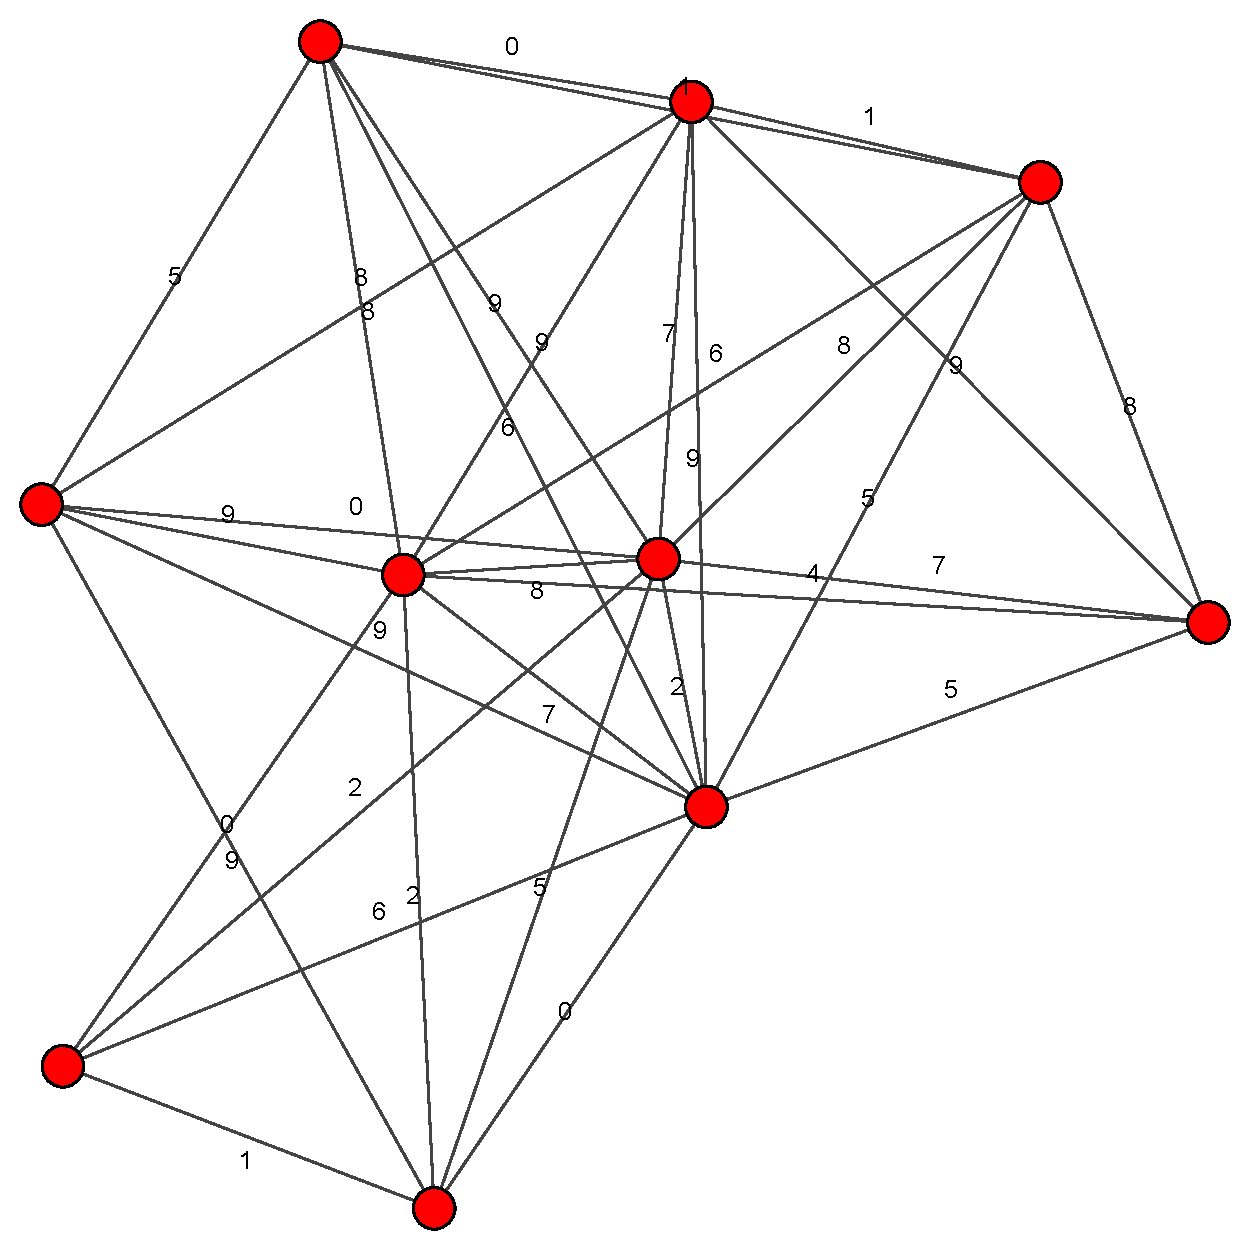
\includegraphics[height=.8\textheight]{fig/mstp-0.pdf}
    \end{center}
\end{frame}
\begin{frame}{Exemple 2 : arbre couvrant minimal (non pondéré)}
    \begin{center}
        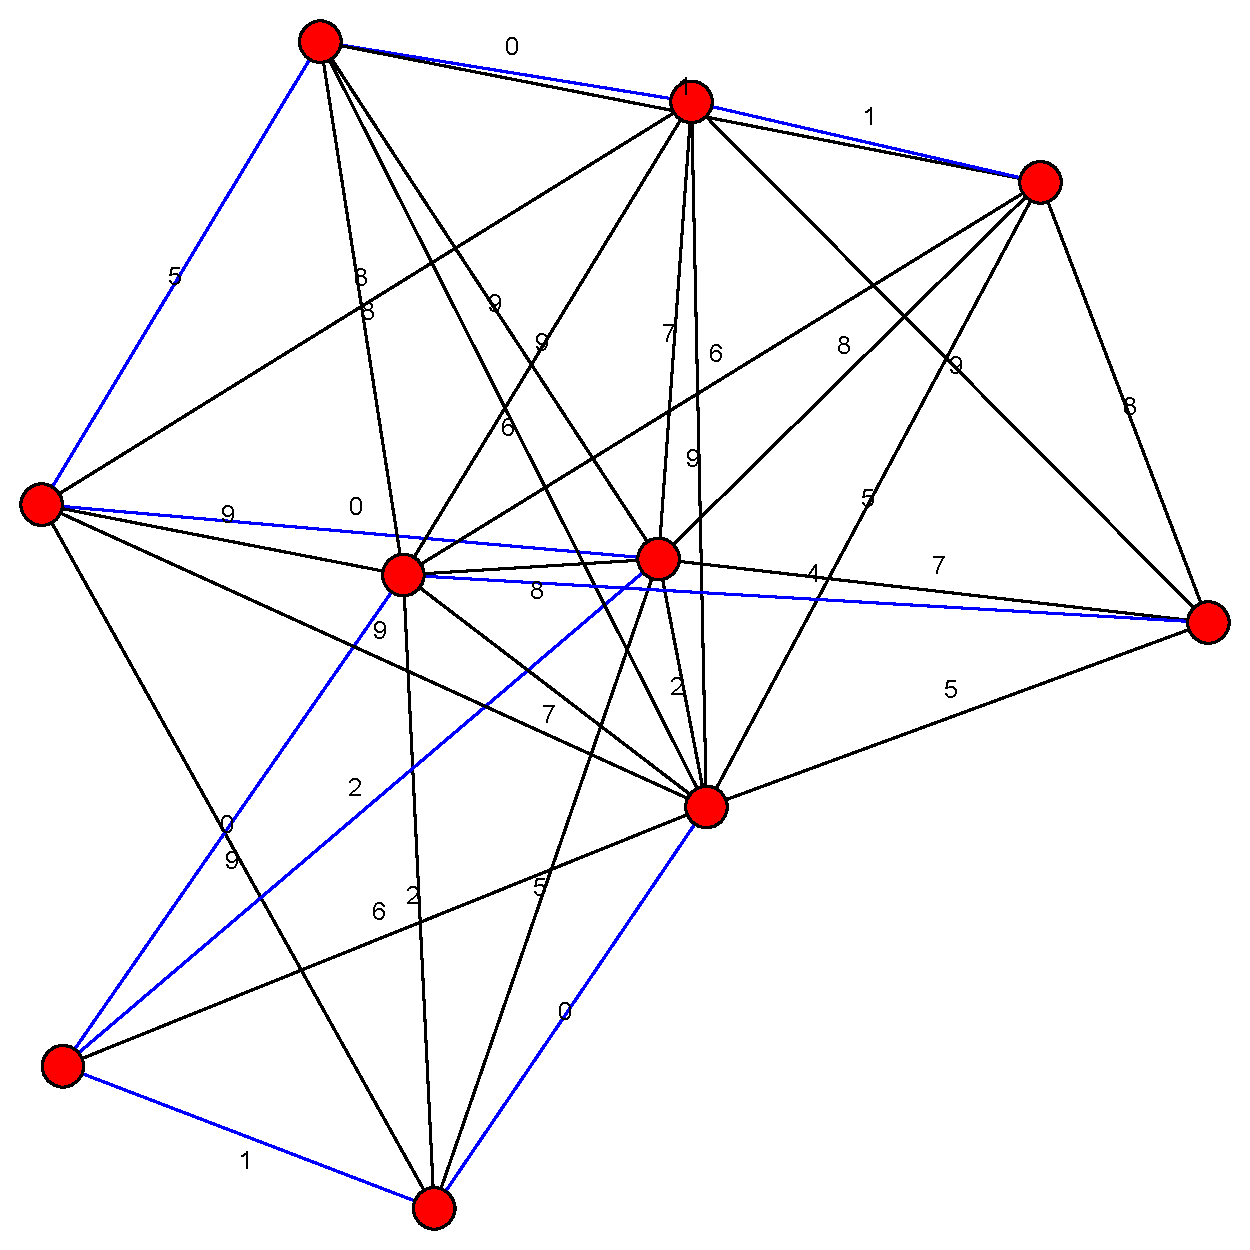
\includegraphics[height=.8\textheight]{fig/mstp-1.pdf}
    \end{center}
\end{frame}

\begin{frame}{Quelques ropriétés}
    \begin{block}{Propriété}
        Ajouter une arête à un graphe non-orienté connexe, crée un cycle
    \end{block}
    L'arête $a$ ajoutée connecte deux sommets $i$ et $j$. Or, le graphe étant connexe, il existait un chemin entre $i$ et $j$ dans le graphe initial. Ajouter $a$ à ce chemin crée un cycle.  
\end{frame}

\begin{frame}{Quelques propriétés}
    \begin{block}{Propriété}
        Enlever une arête à un arbre le rend non-connexe. L'arbre a alors exactement deux composantes connexes. 
    \end{block}
    On note $T-a$ l'arbre privé d'une arête quelconque $a$. On le suppose toujours connexe. Si on ajoute $a$ et qu'on applique la propriété précédente, $T-a$ auquel on a ajouté possède un cycle, ce qui est contradictoire avec le fait que $T$ est un arbre. 
\end{frame}

\begin{frame}{Coupe}
    \begin{definition}
        Une coupe associée à un graphe $G=(S,A)$ est une partition de l'ensemble des sommets $S$ en deux ensembles disjoints $S_1$ et $S_2$. Une arête traversante est une arête $(i,j)$ telle que $i \in S_1$ et $j \in S_2$. 
    \end{definition}
\end{frame}

\begin{frame}{Propriété des cycles}

    \begin{block}{Hypothèse}
        On considère un graphe non-orienté pondéré connexe. On suppose que toutes ses arêtes ont des poids différents
    \end{block}

    Cela assure l'unicité d'un arbre couvrant minimal (admis). Les algorithmes que nous allons voir n'ont pas besoin de cette hypothèse mais l'arbre couvrant minimal n'est plus unique. 
    
    \begin{block}{Propriété}
        Soit $C$ un cycle de $G$. Soit une $f$ une arête de poids maximum dans ce cycle. Alors $f$ n'appartient pas à l'arbre couvrant minimal.
    \end{block}

\end{frame}

\begin{frame}{Démonstration}

    \begin{itemize}
        \item Supposons, par l'absurde que $f$ appartienne à l'arbre couvrant minimal ACM
        \item Enlever $f$ de ACM le coupe en deux composantes connexes 
        \item Il existe une arête $e$ du cycle $C$ qui peut reconnecter les deux composantes 
        \item ACM$-{f}+{e}$ est un nouvel arbre couvrant 
        \item Comme $f$ était l'arête de poids maximum de $C$, ACM$-{f}+{e}$ a un poids inférieur strictement à ACM
        \item Contradiction !
    \end{itemize}
    
\end{frame}

\begin{frame}{Propriété de la coupe}
    
    \begin{block}{Propriété}
        Soit une coupe $S_1,S_2$ de $G$. Soit $e$ l'arête traversante de poids minimum de cette coupe. Alors $e$ appartient forcément à l'arbre couvrant minimal. 
    \end{block}
\end{frame}

\begin{frame}{Démonstration}
    \begin{itemize}
        \item On suppose, par l'absurde, que $e$ n'appartienne pas à l'ACM 
        \item Ajouter $e$ à l'ACM crée alors un cycle 
        \item Il existe une autre arête traversante $f$ qui sépare l'ACM en deux composantes connexes 
        \item ACM$-{f}+{e}$ est nouvel arbre couvrant 
        \item Son poids total est strictement inférieur à celui de ACM 
        \item Contradiction !
    \end{itemize}
\end{frame}


\begin{frame}{Schéma d'un algorithme glouton}
    \begin{itemize}
        \item On colorie toutes les arêtes de $G$ en noir. On va progressivement colorier en rouge les arêtes de l'arbre couvrant minimal 
        \item On choisit une coupe avec aucune arête traversante rouge 
        \item On sélectionne l'arête traversante de poids minimum et on la colorie en rouge 
        \item On répète jusqu'à avoir obtenu l'ACM. Combien d'arêtes faut-il ? 
        \begin{itemize}
            \item l'arbre couvrant minimal comporte $n-1$ arêtes 
        \end{itemize}
    \end{itemize}
\end{frame}

\begin{frame}{Correction de l'algorithme}
    \begin{itemize}
        \item Par propriété de la coupe, toutes les arêtes rouges sont dans ACM 
        \item Tant qu'il y a moins de $n-1$ arêtes rouges, on pourra toujours trouver une coupe 
        \begin{itemize}
            \item tant que la forêt noire n'est pas couvrante, ou pas connexe 
        \end{itemize}
    \end{itemize}
\end{frame}

\directlua{\detokenize{
    for i=1,8,1 do
        tex.sprint("\\begin{frame}{Exemple}\\begin{center} \\includegraphics[height=.8\\textheight]{fig/mst-greedy-", i, ".pdf} \\end{center} \\end{frame}")
    end
}}

\begin{frame}{Les algoroithmes gloutons}
    \begin{itemize}
        \item Approche algorithmique générale pour résoudre des problèmes d'optimisation 
        \item Construction progressive d'une solution 
        \item A chaque étape on fait un choix local optimal, sans se préoccuper de l'effet global
        \item L'approche gloutonne ne fonctionne pas toujours... mais reste simple 
    \end{itemize}
\end{frame}



\begin{frame}{Algorithme de Prim}
    \begin{itemize}
        \item On colorie toutes les arêtes de $G$ en noir. Puis on va progressivement colorier en rouge les arêtes de l'arbre couvrant minimal. A chaque étape le sous-graphe rouge est un arbre. On colorie en rouge les sommets reliés par des arêtes rouges
        \item On choisit un sommet de départ
        \item On considère la coupe distinguant  les sommets rouges des autres. On choisit une arête traversante minimale pour cette coupe et on le colorie en rouge. On colorie également en rouge le sommet qui ne l'était pas encore.
        \item On répète jusqu'à avoir colorié en rouge tous les sommets 
    \end{itemize}
\end{frame}

\begin{frame}{Correction}
\begin{itemize}
    \item A chaque étape, le sous-graphe rouge (sommets et arêtes) est connexe 
    \begin{itemize}
        \item C'est vrai au départ (choix du sommet de départ)
        \item C'est encore vrai après avoir ajouté une arête et un sommet 
    \end{itemize}
    \item A chaque étape, l'arête choisie vérifie les hypothèses de l'algorithme glouton générique 
    \begin{itemize}
        \item C'est l'arête minimum pour la coupe (rouge / pas rouge) courante 
    \end{itemize}
    \item Chaque étape ajoute donc une arête appartenant à l'arbre couvrant minimal 
\end{itemize}
\end{frame}
\directlua{\detokenize{
    for i=0,5,1 do
        tex.sprint("\\begin{frame}{Exemple}\\begin{center} \\includegraphics[height=.8\\textheight]{fig/mstprim-", i, ".pdf} \\end{center} \\end{frame}")
    end
}}

% TODO ajouter l'algorithme de Kruskal (avec Union-Find) ?

\begin{frame}{Longueur d'un chemin}
    \begin{definition}
        Dans un graphe $G=(S,A)$ pondéré (muni d'une fonction $c:A \longrightarrow \mathbf{Z})$, la \emph{longueur} d'un chemin est la somme des poids des arcs le composant 
    \end{definition}
    \begin{definition}
       La \emph{distance minimum} $\delta(i,j)$ entre deux sommets $i$ et $j$ est alors le minimum des longueurs des chemins entre $i$ et $j$ 
    \end{definition}
\begin{definition}
    On appelle \emph{circuit absorbant} un circuit dont la longueur est négative.
\end{definition}
Pour la suite, on pose l'hypothèse que nos graphes n'ont pas de circuit absorbant.

\end{frame}

\begin{frame}{Algorithmes de plus courts chemins}
    \begin{itemize}
        \item Plusieurs questions
        \begin{itemize}
            \item Quel est le plus court chemin de $i$ à $j$?
            \item Quels sont tous les plus courts chemins issus de $i$ ?
            \item Quels sont les plus courts chemins entre tous les sommets du graphe (distancier) ?
        \end{itemize}
        \item Des hypothèses restrictives pour simplifier certains algorithmes
    \end{itemize}
\end{frame}

\begin{frame}{Calcul des plus courts chemins à partir d'une origine}
    \begin{itemize}
        \item Les plus courts chemins issus d'un sommet $s$ forment un \textbf{arbre}
        \begin{itemize}
            \item on suppose que le graphe ne possède pas de circuit absorbant
            \item on suppose également que le graphe est connexe 
        \end{itemize}  
        \item On souhaite alors calculer deux tableaux 
        \begin{itemize}
            \item \texttt{dist[i]} : la distance minimale de $s$ à $i$
            \item \texttt{pred[i]} : le prédécesseur de $i$ dans un chemin minimal de $s$ à $i$
            \begin{itemize}
                \item cela suppose que systématiquement $i$ est un successeur de \texttt{pred[i]}
            \end{itemize}
        \end{itemize}
    \end{itemize}
\end{frame}

\begin{frame}{Calcul des plus courts chemins à partir d'une origine}
    \begin{theorem}
        Si $j$ est un prédécesseur de $i$ dans un chemin minimal de $s$ à $i$, alors $\delta(s,i) = \delta(s,j)+c(j,i)$
    \end{theorem}
        \begin{proof}
            \begin{itemize}
            \item On considère un tel chemin de $s$ à $i$ passant par $j$ puis comprenant l'arc $(j,i)$. Il est de longueur $\delta(s,i)$
            \item Le chemin extrait de $s$ à $j$ est minimal sinon on pourrait construire un chemin de $s$ à $i$ strictement plus court que $\delta(s,i)$
            \item Le chemin considéré de $s$ à $i$ a donc pour longueur $\delta(s,j)+c(j,i)$
            \item Donc, on a bien $\delta(s,i) = \delta(s,j)+c(j,i)$
        \end{itemize}
    \end{proof}
\end{frame}


\begin{frame}{Calcul des plus courts chemins à partir d'une origine}
    \begin{theorem}
        le graphe formé par la relation \texttt{pred} est un \arbre
    \end{theorem}
        \begin{proof}
            \begin{itemize}
                \item S'il existait un cycle passant par un sommet $i$, cela signifierait qu'il existe un plus court chemin de $s$ à $i$, passant par $i$ et par $s$ lui-même. $s$ ne pouvant pas avoir de prédécesseur, le graphe est donc acyclique 
            \item Pour l'instant, nous savons que le graphe est une \foret. Si un arbre de cette forêt n'avait pas $s$ pour racine, cela signifierait qu'il n'y a pas de chemin minimal de $s$ à cette racine dans le graphe de départ. C'est en contradiction avec l'hypothèse, donc le graphe est connexe
            \item Le graphe étant connexe et acyclique, c'est un arbre 
        \end{itemize}
    \end{proof}
\end{frame}

\begin{frame}{Algorithme ordinal}
    \begin{itemize}
        \item On se restreint à un \textbf{graphe acylique}
        \item On parcourt le graphe selon un ordre topologique
        \item A chaque étape, on examine le sommet $i$, sous condition qu'on ait calculé \texttt{dist[j]} pour tous les prédécesseurs $j$ de $i$ dans le graphe 
        \item On calcule alors 

        $$
        \mathtt{dist}[i] = \min \{  \mathtt{dist}[j] + c(j,i), j \in \Gamma^{-}(j)\}
        $$
    \end{itemize}
\end{frame}

\begin{frame}[fragile]
    \frametitle{Algorithme ordinal : version en arrière}
    \begin{algorithmic}[1]
        \Function{ordinal}{$G$,$s$}
        \State ord \gets tri\_topologique($G$)
        \State dist \gets [$\infty,...,\infty$] 
        \For{k $\in [0,...n-1]$}
            \State i \gets ord[k]
            \If{i=s}
                dist[i] \gets 0
            \Else
                \For{j $\in \Gamma^{-1}(j)$}
                    \If{dist[j]+c(j,i) < dist[i]}
                        \State dist[i] \gets  dist[j]+c(j,i)
                        \State pred[i] \gets j
                    \EndIf
                \EndFor 
            \EndIf  
        \EndFor
        \EndFunction
    \end{algorithmic}
\end{frame}

\begin{frame}{Tri topologique}
    \begin{definition}
        Un \emph{tri topologique} est un ordre total sur l'ensemble des sommets dans lequel $s$ précède $t$ pour tout arc d'un sommet $s$ vers un sommet $t$
    \end{definition}
    \begin{itemize}
        \item Plusieurs algorithmes pour obtenir un tri topologique
        \begin{itemize}
            \item parcours en profondeur pendant lequel on empile chaque sommet une fois tous ses successeurs visités. En désempilant, on obtient un tri topologique
            \item On peut aussi chercher une racine (sommet sans prédécesseur), l'enlever et répéter l'opération autant de fois que nécessaire
        \end{itemize}
        \item Remarque : il n'existe pas d'ordre topologique unique pour un graphe 
    \end{itemize}
\end{frame}

\begin{frame}{Exemple}
    \begin{center}
        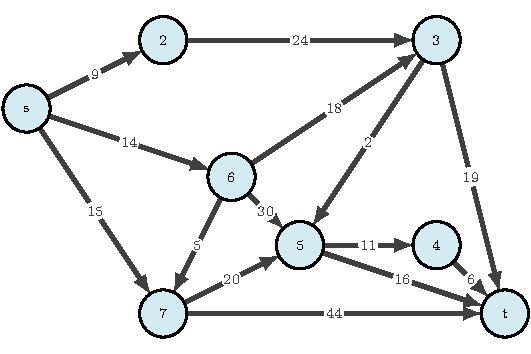
\includegraphics[height=.6\textheight]{fig/ordinal-0.pdf}

        Ordre topologique : $s,6,7,2,3,5,4,t$
    \end{center}
\end{frame}

\begin{frame}{Itérations de l'algorithme : traitement de $s$}
    \begin{center}
        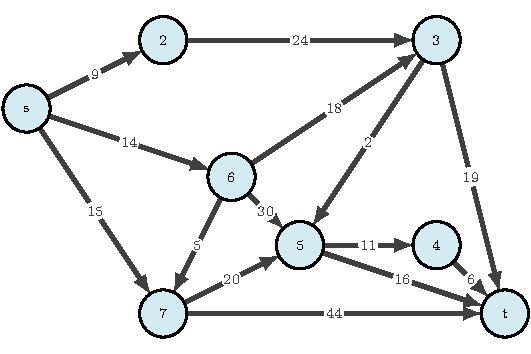
\includegraphics[height=.6\textheight]{fig/ordinal-0.pdf}      
    \begin{tabular}{c|cccccccc}
        
        sommet & s       &2      &7      &6      &5      &3      &4      &t      \\
        \hline
        \texttt{pred} & &       &       &       &       &       &       &       \\
        \texttt{dist} & 0       &inf    &inf    &inf    &inf    &inf    &inf    &inf    \\
    \end{tabular}
\end{center}
\end{frame}

\begin{frame}{Itérations de l'algorithme : traitement de $6$}
    \begin{center}
        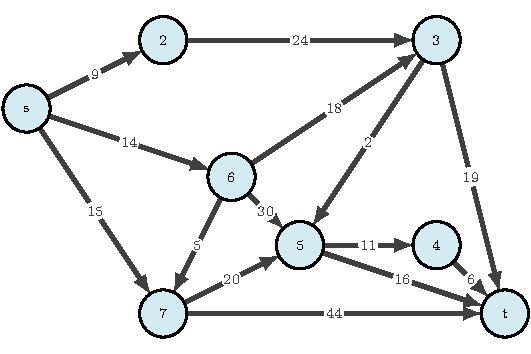
\includegraphics[height=.6\textheight]{fig/ordinal-0.pdf}      
    \begin{tabular}{c|cccccccc}
        
        sommet & s       &2      &7      &6      &5      &3      &4      &t      \\
        \hline
        \texttt{pred} & &       &       &s      &       &       &       &       \\
        \texttt{dist} & 0       &inf    &inf    &14     &inf    &inf    &inf    &inf    \\
    \end{tabular}
\end{center}
\end{frame}

\begin{frame}{Itérations de l'algorithme : traitement de $7$}
    \begin{center}
        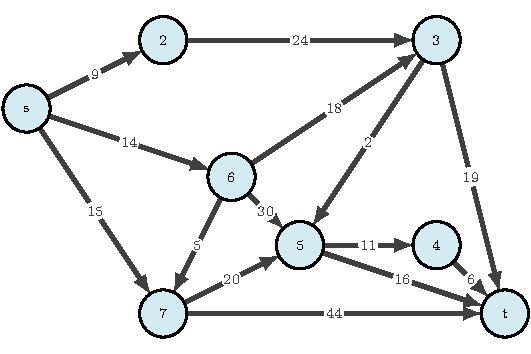
\includegraphics[height=.6\textheight]{fig/ordinal-0.pdf}      
    \begin{tabular}{c|cccccccc}
        
        sommet & s       &2      &7      &6      &5      &3      &4      &t      \\
        \hline
        \texttt{pred} & &       &s      &s      &       &       &       &       \\
        \texttt{dist} & 0       &inf    &15     &14     &inf    &inf    &inf    &inf    \\
    \end{tabular}
\end{center}
\end{frame}

\begin{frame}{Itérations de l'algorithme : traitement de $2$}
    \begin{center}
        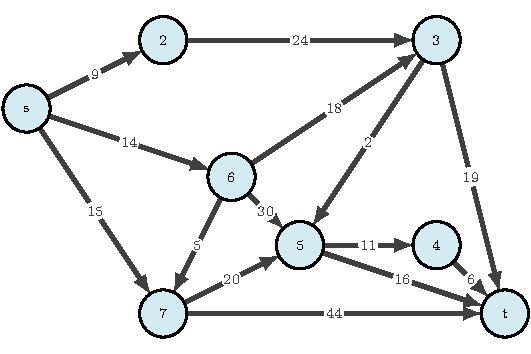
\includegraphics[height=.6\textheight]{fig/ordinal-0.pdf}      
    \begin{tabular}{c|cccccccc}
        
        sommet & s       &2      &7      &6      &5      &3      &4      &t      \\
        \hline
        \texttt{pred} & &s      &s      &s      &       &       &       &       \\
        \texttt{dist} & 0       &9      &15     &14     &inf    &inf    &inf    &inf    \\
    \end{tabular}
\end{center}
\end{frame}

\begin{frame}{Itérations de l'algorithme : traitement de $3$}
    \begin{center}
        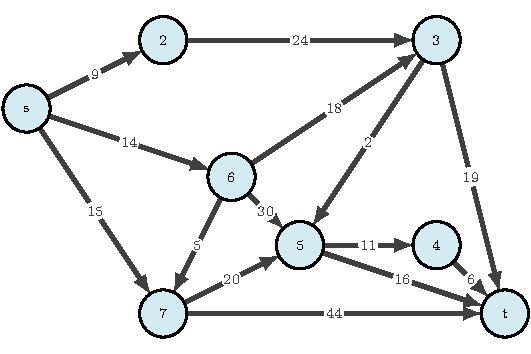
\includegraphics[height=.6\textheight]{fig/ordinal-0.pdf}      
    \begin{tabular}{c|cccccccc}
        
        sommet & s       &2      &7      &6      &5      &3      &4      &t      \\
        \hline
        \texttt{pred} & &s      &s      &s      &       &6      &       &       \\
        \texttt{dist} & 0       &9      &15     &14     &inf    &32     &inf    &inf    \\
    \end{tabular}
\end{center}
\end{frame}

\begin{frame}{Itérations de l'algorithme : traitement de $5$}
    \begin{center}
        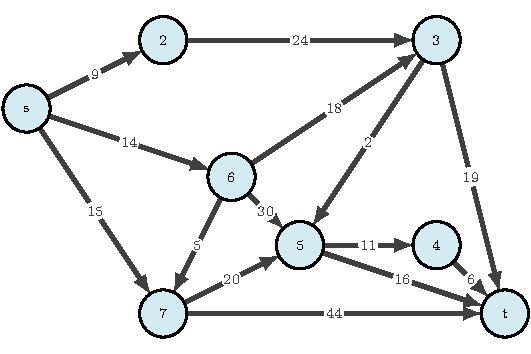
\includegraphics[height=.6\textheight]{fig/ordinal-0.pdf}      
    \begin{tabular}{c|cccccccc}
        
        sommet & s       &2      &7      &6      &5      &3      &4      &t      \\
        \hline
        \texttt{pred} & &s      &s      &s      &3      &6      &       &       \\
        \texttt{dist} & 0       &9      &15     &14     &34     &32     &inf    &inf    \\
    \end{tabular}
\end{center}
\end{frame}

\begin{frame}{Itérations de l'algorithme : traitement de $4$}
    \begin{center}
        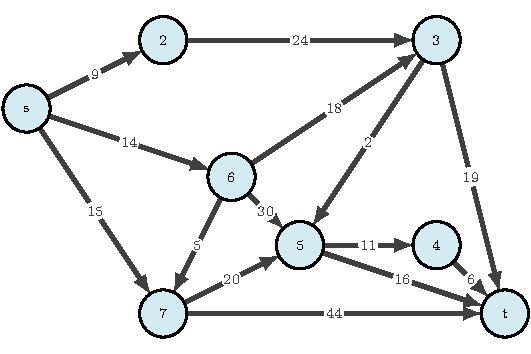
\includegraphics[height=.6\textheight]{fig/ordinal-0.pdf}      
    \begin{tabular}{c|cccccccc}
        
        sommet & s       &2      &7      &6      &5      &3      &4      &t      \\
        \hline
        \texttt{pred} & &s      &s      &s      &3      &6      &5      &       \\
        \texttt{dist} & 0       &9      &15     &14     &34     &32     &45     &inf    \\
    \end{tabular}
\end{center}
\end{frame}

\begin{frame}{Itérations de l'algorithme : traitement de $t$}
    \begin{center}
        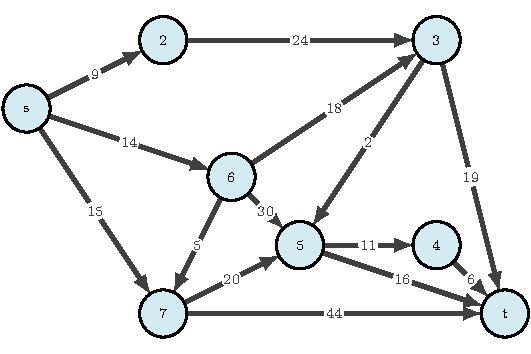
\includegraphics[height=.6\textheight]{fig/ordinal-0.pdf}      
    \begin{tabular}{c|cccccccc}
        
        sommet & s       &2      &7      &6      &5      &3      &4      &t      \\
        \hline
        \texttt{pred} & &s      &s      &s      &3      &6      &5      &5      \\
        \texttt{dist} & 0       &9      &15     &14     &34     &32     &45     &50     \\
    \end{tabular}
\end{center}
\end{frame}


\begin{frame}{Algorithme de Dijkstra}
    \begin{itemize}
        \item On autorise que le graphe contienne des cycles
        \item On se restreint à un \textbf{graphe sans poids négatifs}
        \item Idée : on construit progressivement un ensemble $S$ qui contient les sommets dont nous aurons déjà calculé la distance minimale 
        \item En choisissant à chaque itération un nouveau sommet dont le coût d'accès est minimal qu'on ajoute dans $S$, cette propriété est conservée et on va mettre à jour \texttt{pred} et \texttt{dist} pour les autres sommets
    \end{itemize}
\end{frame}

\begin{frame}[fragile]
    \frametitle{Algorithme}
    \begin{algorithmic}[1]
        \Function{Dijkstra}{$G,s$}
            \State dist \gets [0,$\infty$,...,$\infty$]
            \State $P$ \gets $S$, $T$ \gets $\{\}$
            \While{$T$ non vide}
                \State Choisir $x_0 \in T$ tel que \texttt{dist} minimal
                \State $T$ \gets $T-\{ x_0 \}$, $P$ \gets $P \cup \{ x_0 \}$  
                \For{$j \in \Gamma^+(i)$}
                    \If{dist[i]+c(i,j) < dist[j]}
                        \State dist[j] \gets dist[i]+c(i,j)
                        \State pred[j] \gets i
                    \EndIf 
                \EndFor
            \EndWhile
        \EndFunction
    \end{algorithmic}
\end{frame}


\begin{frame}{Exemple}
    \begin{center}
        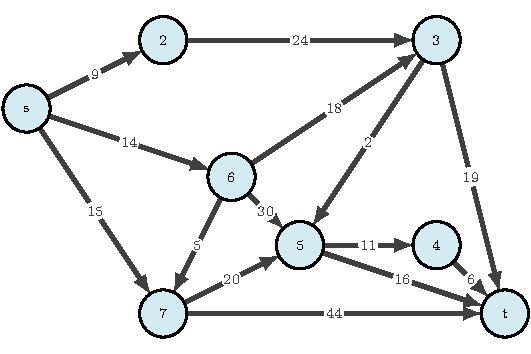
\includegraphics[height=.6\textheight]{fig/dijkstra-0.pdf}

    \end{center}
\end{frame}

\begin{frame}{Itérations de l'algorithme : traitement de $s$}
    \begin{center}
        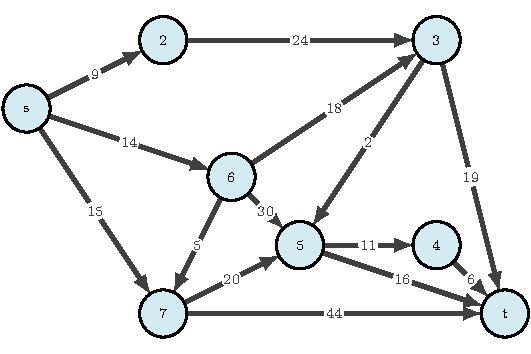
\includegraphics[height=.6\textheight]{fig/dijkstra-0.pdf}      
    \begin{tabular}{c|cccccccc}
      
        & \textbf{s}   &2      &7      &6      &5      &3      &4      &t      \\
        \hline
        \texttt{pred} & &s      &s      &s      &       &       &       &       \\
        \texttt{dist} & 0       &9      &15     &14     &$+\infty$    &$+\infty$    &$+\infty$    &$+\infty$    \\
            \end{tabular}
\end{center}
\end{frame}


\begin{frame}{Itérations de l'algorithme : traitement de $2$}
    \begin{center}
        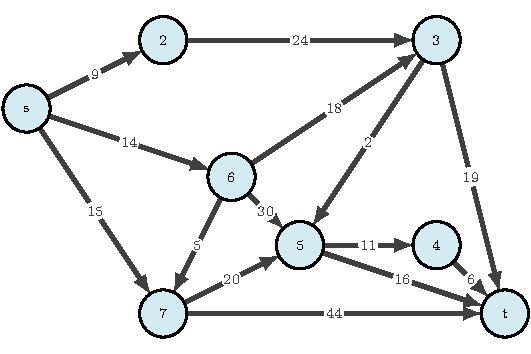
\includegraphics[height=.6\textheight]{fig/dijkstra-0.pdf}      
    \begin{tabular}{c|cccccccc}
      
        & \textbf{s}   &\textbf{2}     &7      &6      &5      &3      &4      &t      \\
        \hline
        \texttt{pred} & &s      &s      &s      &       &2      &       &       \\
        \texttt{dist} & 0       &9      &15     &14     &$+\infty$    &33     &$+\infty$    &$+\infty$    \\
                   \end{tabular}
\end{center}
\end{frame}

\begin{frame}{Itérations de l'algorithme : traitement de $6$}
    \begin{center}
        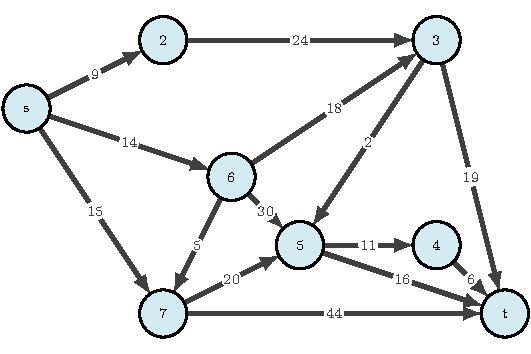
\includegraphics[height=.6\textheight]{fig/dijkstra-0.pdf}      
    \begin{tabular}{c|cccccccc}
      
        & \textbf{s}   &\textbf{2}     &7      &\textbf{6}     &5      &3      &4      &t      \\
        \hline
        \texttt{pred} & &s      &s      &s      &6      &6      &       &       \\
        \texttt{dist} & 0       &9      &15     &14     &44     &32     &$+\infty$    &$+\infty$    \\
                           \end{tabular}
\end{center}
\end{frame}


\begin{frame}{Itérations de l'algorithme : traitement de $7$}
    \begin{center}
        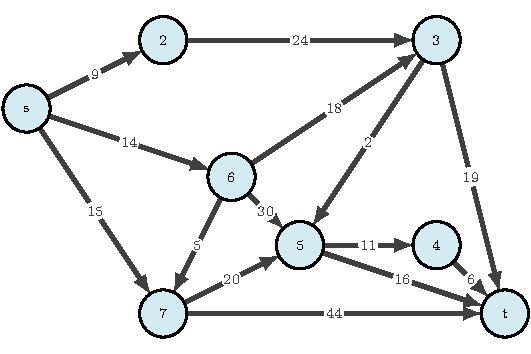
\includegraphics[height=.6\textheight]{fig/dijkstra-0.pdf}      
    \begin{tabular}{c|cccccccc}
      
        & \textbf{s}   &\textbf{2}     &\textbf{7}     &\textbf{6}     &5      &3      &4      &t      \\
        \hline
        \texttt{pred} & &s      &s      &s      &7      &6      &       &7      \\
        \texttt{dist} & 0       &9      &15     &14     &35     &32     &$+\infty$    &59     \\
    \end{tabular}
\end{center}
\end{frame}

\begin{frame}{Itérations de l'algorithme : traitement de $3$}
    \begin{center}
        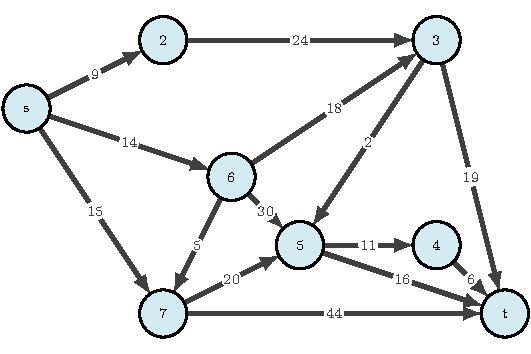
\includegraphics[height=.6\textheight]{fig/dijkstra-0.pdf}      
    \begin{tabular}{c|cccccccc}
      
        & \textbf{s}   &\textbf{2}     &\textbf{7}     &\textbf{6}     &5      &\textbf{3}     &4      &t      \\
        \hline
        \texttt{pred} & &s      &s      &s      &3      &6      &       &3      \\
        \texttt{dist} & 0       &9      &15     &14     &34     &32     &$+\infty$    &51     \\
    \end{tabular}
\end{center}
\end{frame}

\begin{frame}{Itérations de l'algorithme : traitement de $5$}
    \begin{center}
        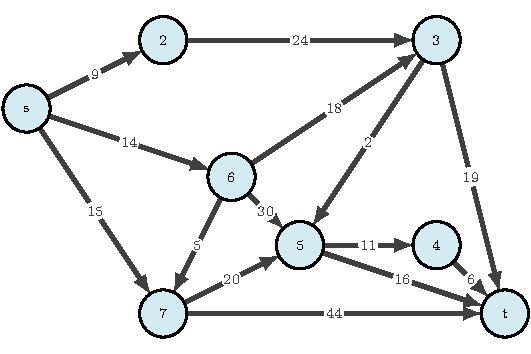
\includegraphics[height=.6\textheight]{fig/dijkstra-0.pdf}      
    \begin{tabular}{c|cccccccc}
      
        & \textbf{s}   &\textbf{2}     &\textbf{7}     &\textbf{6}     &\textbf{5}     &\textbf{3}     &4      &t      \\
        \hline
        \texttt{pred} & &s      &s      &s      &3      &6      &5      &5      \\
        \texttt{dist} & 0       &9      &15     &14     &34     &32     &45     &50     \\
            \end{tabular}
\end{center}
\end{frame}


\begin{frame}{Itérations de l'algorithme : traitement de $4$}
    \begin{center}
        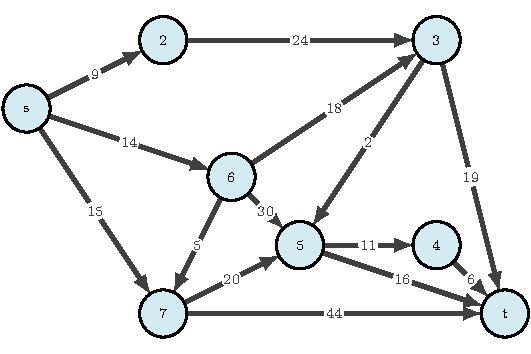
\includegraphics[height=.6\textheight]{fig/dijkstra-0.pdf}      
    \begin{tabular}{c|cccccccc}
      
        & \textbf{s}   &\textbf{2}     &\textbf{7}     &\textbf{6}     &\textbf{5}     &\textbf{3}     &\textbf{4}     &t      \\
        \hline
        \texttt{pred} & &s      &s      &s      &3      &6      &5      &5      \\
        \texttt{dist} & 0       &9      &15     &14     &34     &32     &45     &50     \\
                \end{tabular}
\end{center}
\end{frame}

\begin{frame}{Fin de l'algorithme}
    \begin{center}
        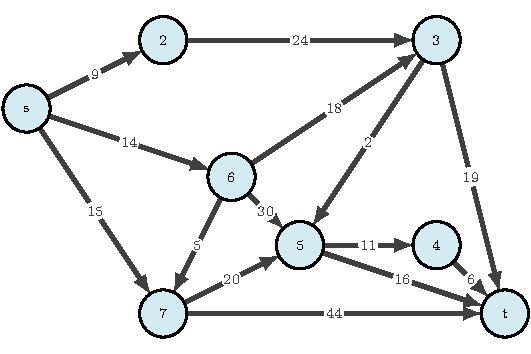
\includegraphics[height=.6\textheight]{fig/dijkstra-0.pdf}      
    \begin{tabular}{c|cccccccc}
      
        & \textbf{s}   &\textbf{2}     &\textbf{7}     &\textbf{6}     &\textbf{5}     &\textbf{3}     &\textbf{4}     &\textbf{t}     \\
        \hline
        \texttt{pred} & &s      &s      &s      &3      &6      &5      &5      \\
        \texttt{dist} & 0       &9      &15     &14     &34     &32     &45     &50     \\
                        \end{tabular}
\end{center}
\end{frame}








% Algorithmes de flot 
\section{Algorithmes de flot maximal}
% algorithmes de flot max




\end{document}
